%
%  愛知工業大学経営情報科学部情報科学科
%    コンピュータシステム専攻用LaTeXテンプレート(2015.12.22)
%
\documentclass{jbook}
% 使いたい人は使う
\usepackage{personal}
% 図挿入用
\usepackage{graphicx}
\usepackage{latexsym}
\usepackage{amssymb}
\usepackage{amsfonts}
\usepackage{ulinej}
\usepackage{url}
\pagestyle{headings}

% カウンタセット
\setcounter{secnumdepth}{3}
\setcounter{tocdepth}{3}
% 定義環境
\newtheorem{definition}{定義}[section]
% 例環境
\newtheorem{example}{例}[section]
% 新しい環境の定義
\newenvironment{indention}[1]{\par
\addtolength{\leftskip}{#1}
\begingroup}{\endgroup\par}
% 関連図書→参考文献
\renewcommand{\bibname}{参考文献}

\topmargin=-14mm
\headsep=15mm
\textwidth=15.7cm
%\baselineskip=22pt
%\renewcommand{\baselinestretch}{1.4}
\textheight=24.5cm  % 33 lines in 1 page
\oddsidemargin=7.5mm
\evensidemargin=7.5mm

% 部分コンパイル用
%\includeonly{title,chap1,chap2,chap3,chap4,chap5,thanks,reference}
\begin{document}

\begin{titlepage}

\ \\
\begin{center}

{\LARGE 愛知工業大学情報科学部情報科学科\\
メディア情報専攻

\vspace{1.0cm}

平成30年度~卒業論文\\

\vspace{2.0cm}

{\Huge 
\baselineskip=15mm
\textbf{\\認知症予防トレーニングの\\負荷調整システムに関する研究\\}}

\vspace{5.0cm}

2018年2月\\

\vspace{1.0cm}

\begin{tabular}[h]{lll}
  研究者 & X13001 & 相羽瑛仁\\
\end{tabular}

\vspace{1.0cm}

指導教員\ \ 澤野弘明\ \ 准教授}

\end{center}

\end{titlepage}
%%% Local Variables: 
%%% mode: latex
%%% TeX-master: "root"
%%% End: 


%目次を自動的に作る。
\tableofcontents

% 本文

\chapter{緒言}
\thispagestyle{myheadings}

\section{背景}
認知症とは,記憶,判断などの認知機能が後天的な脳の障害によって持続的に低下し,日常生活に支障をきたす状態である\cite{認知症とは}.認知症は加齢に伴う病気であり,高齢者数の増大とともに,認知症の有病者数は増大する\cite{認知症予防マニュアル}.内閣府による65歳以上の認知症高齢者数の調査\cite{高齢社会白書}では,図\ref{fig:dementia_senior_number}に示すように平成24年は426万人,平成37年は推計で約700万人になると報告されており,認知症の発症および進行を遅らせる予防の重要性が増している\cite{新オレンジプラン}.認知症予防の方法には社会参加,対人交流,運動の実施などが挙げられ\cite{運動の効果},特に運動は,地方自治体によって高齢者向けの運動教室が広く展開されている.\cite{運動教室}.

運動教室で実施される認知症予防を目的としたトレーニングの一つにコグニサイズ(cognicise)がある\cite{コグニサイズとは}.コグニサイズは国立長寿医療研究センター\cite{国立長寿医療研究センター}が開発したトレーニングであり,運動と同時に,計算やしりとりなどの認知課題を行う.運動教室でのコグニサイズの実施の様子を図\ref{fig:20171207_cognicise}に示す.コグニサイズは実施する運動と認知課題に応じて,コグニステップ,コグニラダー,コグニウォークなどの種類があり,これらを総称してコグニサイズとしている\cite{認知症予防へ向けた運動コグニサイズ}.例えばコグニステップでは,数字を数えながら左右の足で交互にステップをする運動と同時に,一定間隔ごとの決められた数字で拍手をする認知課題を行う.コグニステップの実施方法を図\ref{fig:cognistep}に示す.文献\cite{コグニサイズとは}では,認知症予防の効果があるコグニサイズの条件として,1)運動は全身を使った中強度程度の負荷がかかるものであり,脈拍数が上昇する,2)運動と同時に実施する認知課題によって,運動の方法や認知課題自体をたまに間違えてしまう程度の負荷がかかっているとしている.また文献\cite{認知症予防へ向けた運動コグニサイズ}では,個人の身体状況に応じて,運動と認知課題の負荷を調整することが重要だとしている.しかし,運動教室で実施される集団でのコグニサイズは,参加者全員に対する負荷が一定のため,認知症予防の効果が低い参加者が現れる可能性がある\cite{運動教室の効果}.

そこで本研究では,ICT (Information and Communication Technology)を使用し,運動教室で実施される集団でのコグニサイズにおいて,認知課題の負荷を個別に調整する支援を行う.認知課題の正答率を蓄積し,蓄積した認知課題の正答率に応じて,認知課題の負荷を調整可能なシステムを開発する.運動教室の参加者が提案システムを使用することによって,個別に認知症予防の効果があるコグニサイズを実施できることが期待される.

\begin{figure}[tbp]
	\centering
			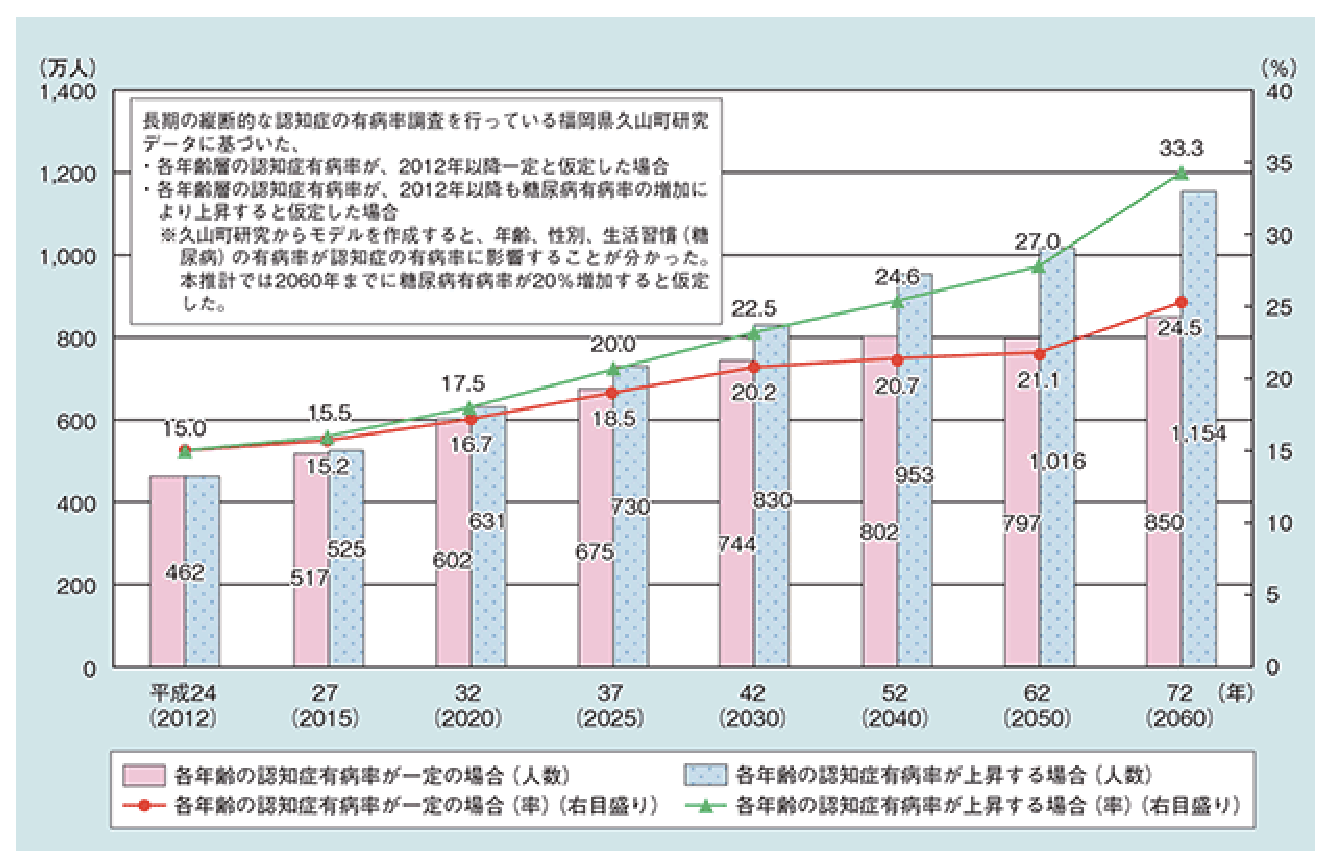
\includegraphics[width=0.9\textwidth]{chap1-figure/dementia_senior_number.eps}
	\caption{認知症高齢者数(文献\cite{高齢社会白書}より引用)}
	\label{fig:dementia_senior_number}
\end{figure}

\begin{figure}[tbp]
	\centering
			\includegraphics[width=0.9\textwidth]{chap1-figure/20171207_cognicise.eps}
	\caption{運動教室でのコグニサイズの実施の様子}
	\label{fig:20171207_cognicise}
\end{figure}

\begin{figure}[tbp]
	\centering
			\includegraphics[width=0.9\textwidth]{chap1-figure/cognistep.eps}
	\caption{コグニステップの実施方法(文献\cite{認知症予防へ向けた運動コグニサイズ}より引用)}
	\label{fig:cognistep}
\end{figure}


\section{関連研究}
本節では,ICTを使用した認知症予防の支援に関する研究について述べる.北越の研究\cite{記憶力ゲーム}では,タブレット端末上に自律的に動作するエージェントを実装し,高齢者がエージェントとの認知課題ゲームに取り組むことで,認知機能の向上を支援するシステムを開発している.認知課題ゲームの画面例を図\ref{fig:cognition_system}に示す.認知課題に視覚的フィードバックを導入することで,高齢者が認知課題に取り組むモチベーションの向上に効果があると報告されている.そのことから,提案システムに認知課題の視覚的フィードバックを導入することで,コグニサイズのモチベーションの向上が期待される.



\begin{figure}[tbp]
	\centering
			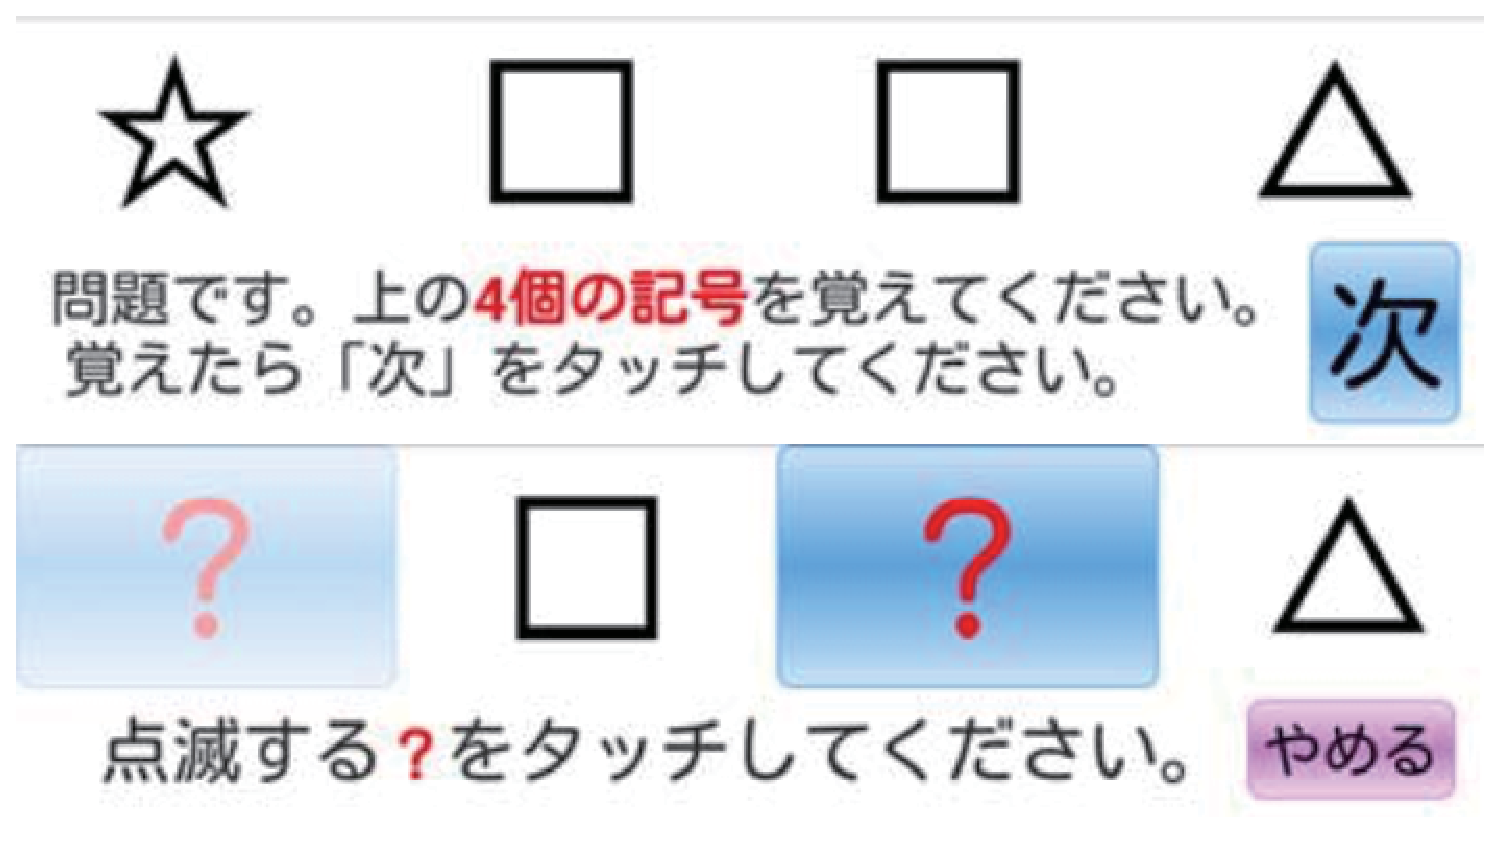
\includegraphics[width=0.7\textwidth]{chap1-figure/cognition_system.eps}
	\caption{認知課題ゲームの画面例(文献\cite{記憶力ゲーム}より引用)}
	\label{fig:cognition_system}
\end{figure}

\begin{figure}[tbp]
	\centering
			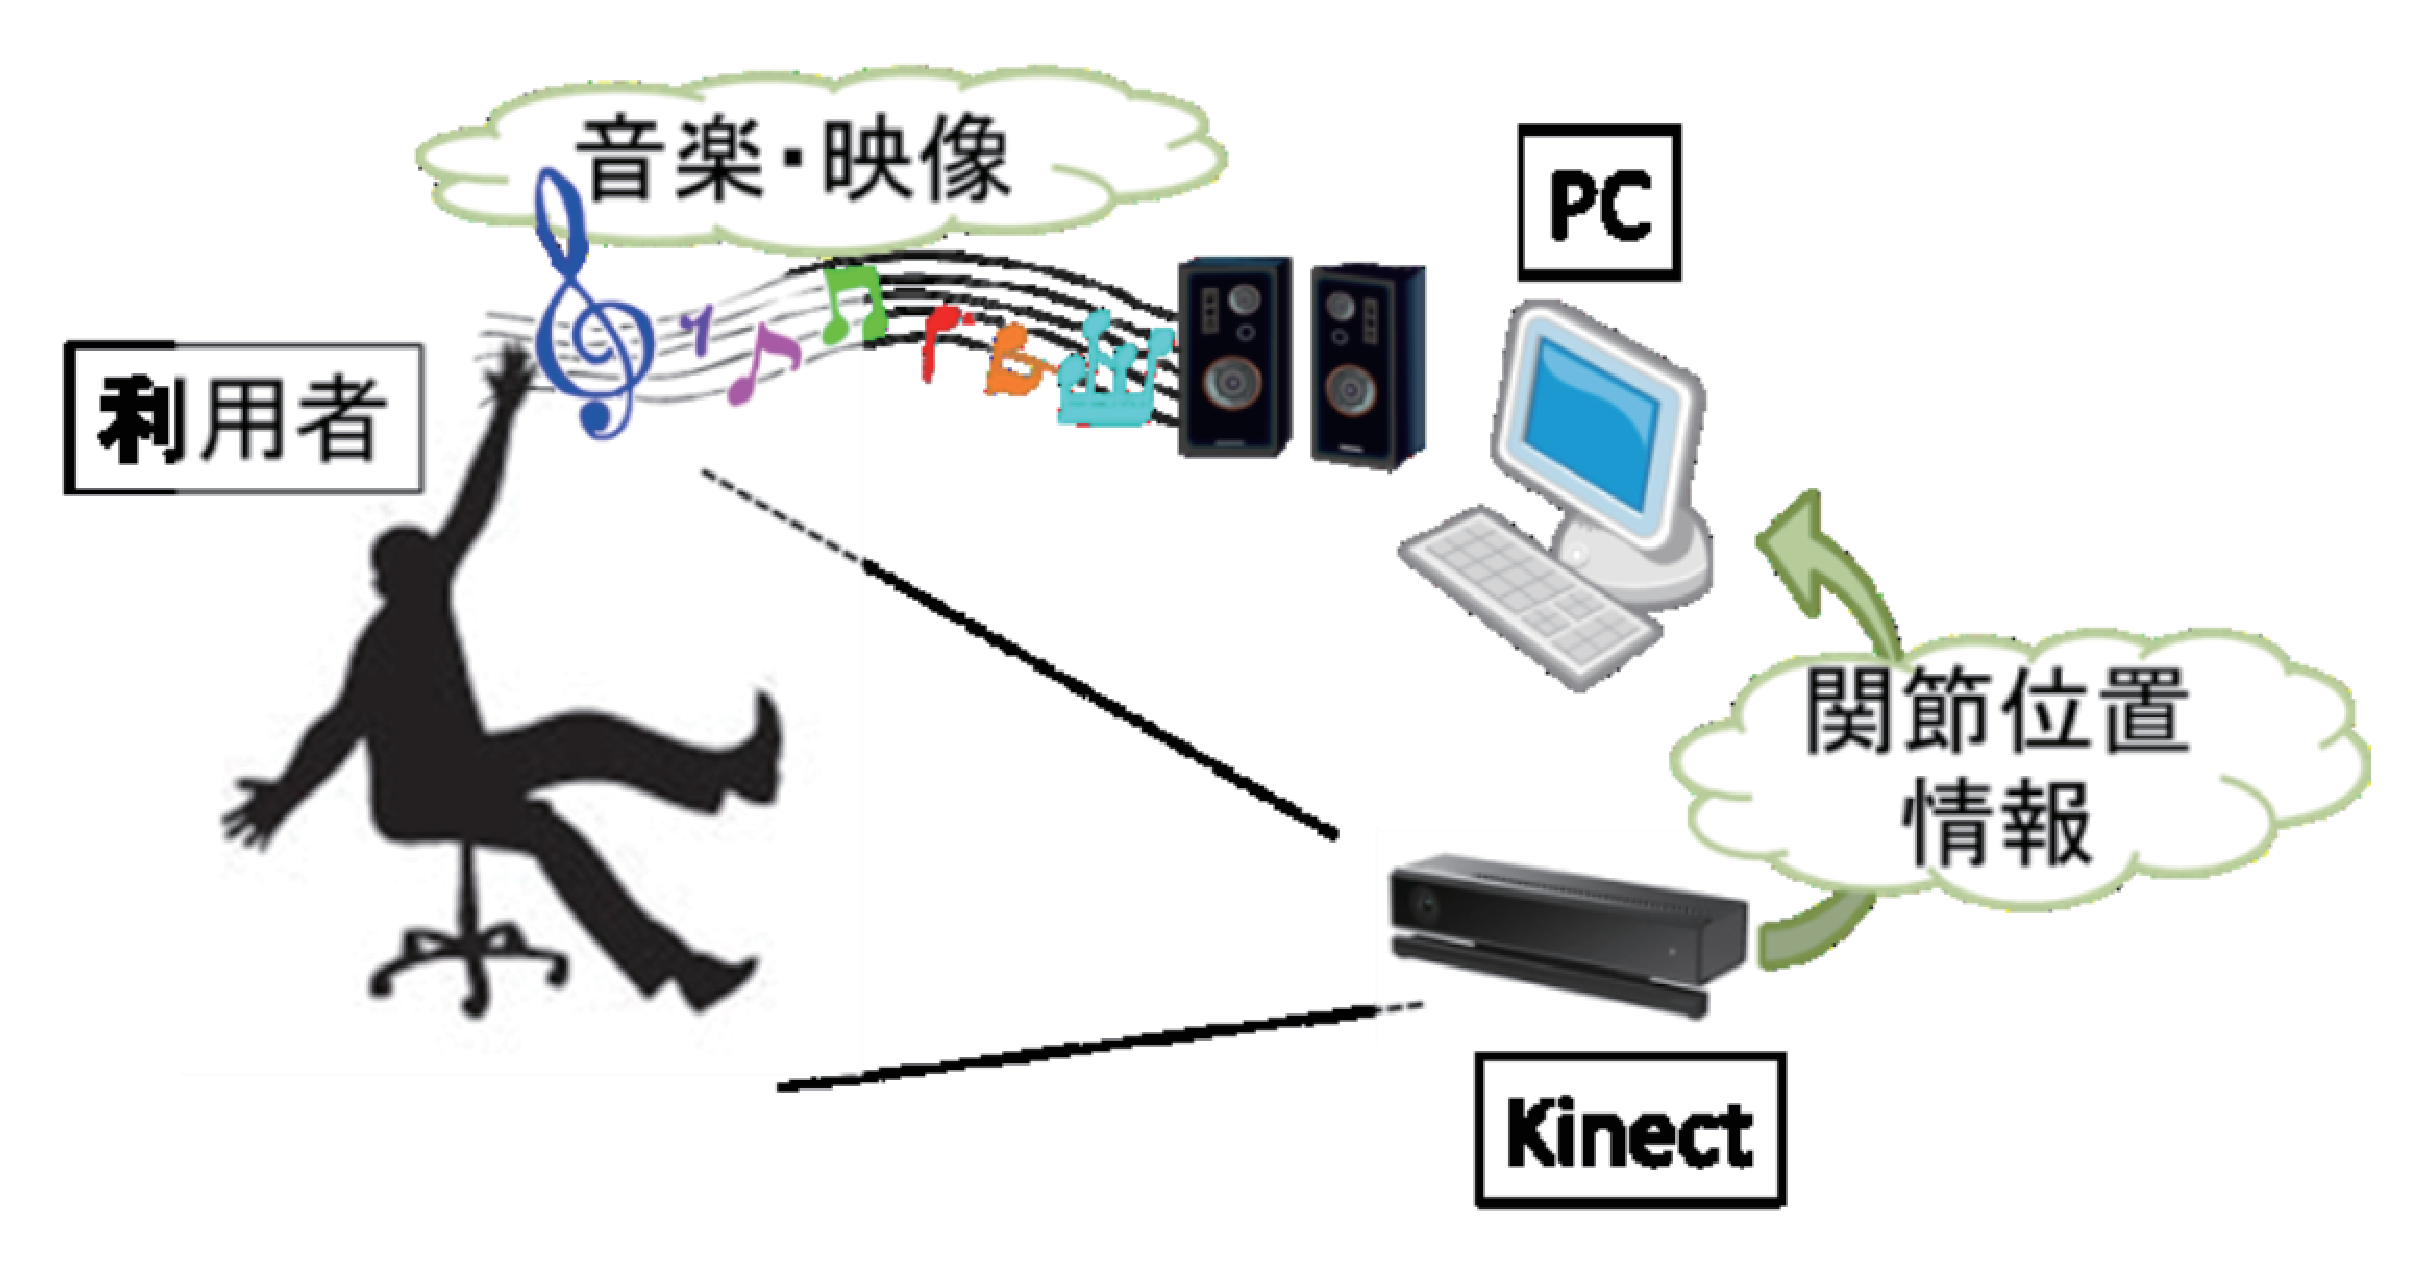
\includegraphics[width=0.7\textwidth]{chap1-figure/antagonism_system.eps}
	\caption{拮抗体操支援システムの概要(文献より引用)}
	\label{fig:antagonism_system}
\end{figure}

\begin{figure}[tbp]
	\centering
			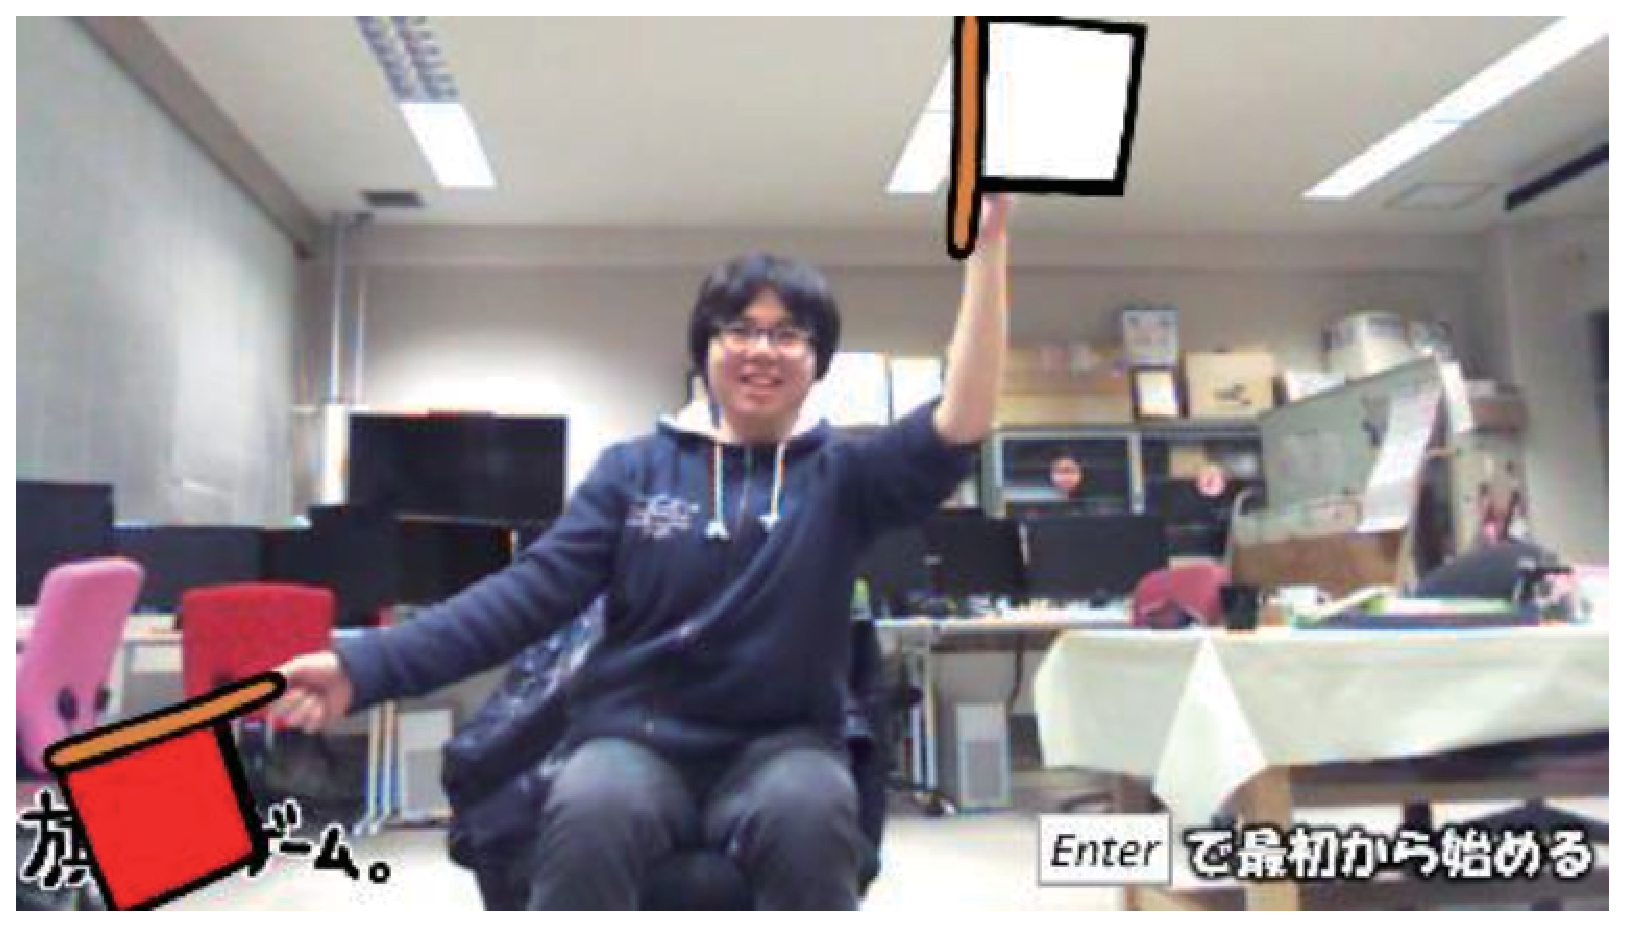
\includegraphics[width=0.7\textwidth]{chap1-figure/upper_limbs_system.eps}
	\caption{レクリエーションゲームの画面例(文献より引用)}
	\label{fig:upper_limbs_system}
\end{figure}


\if0
本節では,機械を使用した下肢リハビリに関する研究と歩行感覚提示装置に使用するディスプレイに関する印象調査に関連する研究について述べる.維持期脳卒中患者に対して歩行感覚提示装置を用いた歩行トレーニングを行い,その効果の持続性の検討\cite{筑波歩行感覚提示}が田中らによって行われている.棚からの歩行感覚提示装置を図\ref{fig:tukuba}に示す.歩行感覚提示装置は,通常の歩行に近い動作かつ,通常の歩行と同じ1m/sの歩行速度を実現可能な装置である.患者は球面型ディスプレイ内を歩く構造となっている.入院前の健康状態の歩幅で自宅付近を歩く疑似体験をすることで,患者自身が早く治したいという気持ちになり,リハビリに対するモチベーションが向上するという精神面での効果も報告されている.しかし,寝たきりの患者は対象とされていない問題点がある.
\fi

\if0
\begin{figure}[tbp]
	\centering
			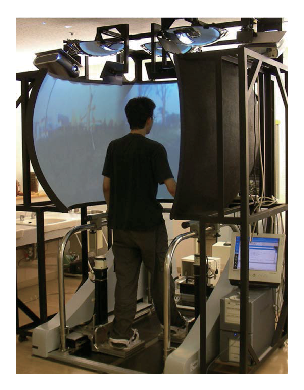
\includegraphics[width=0.5\textwidth]{chap1-figure/tukuba.eps}
	\caption{没入型歩行感覚提示装置全景(文献\cite{筑波歩行感覚提示画像}より引用)}
	\label{fig:tukuba}
\end{figure}

高齢者の自立・社会参加の前提となる歩行機能および歩行訓練に着目し,バーチャルリアリティ(VR: Virtual Reality)を活用した歩行訓練器具\cite{日立}が藤江らによって開発されている.藤江らによる歩行訓練機器を図\ref{fig:hitachi}に示す.リハビリ患者の歩行機能の改善を目指し,自立歩行によって実写映像が切り替わるシステムとなっている.VRを活用しリハビリ患者の訓練意欲を高める試みがされている.リハビリ患者に対して,立体視可能な映像を流した結果,映像に集中していたという結果が報告されている.そのことから,HMDを使用することがリハビリへの集中に繋がることも期待される.

\begin{figure}[tbp]
	\centering
			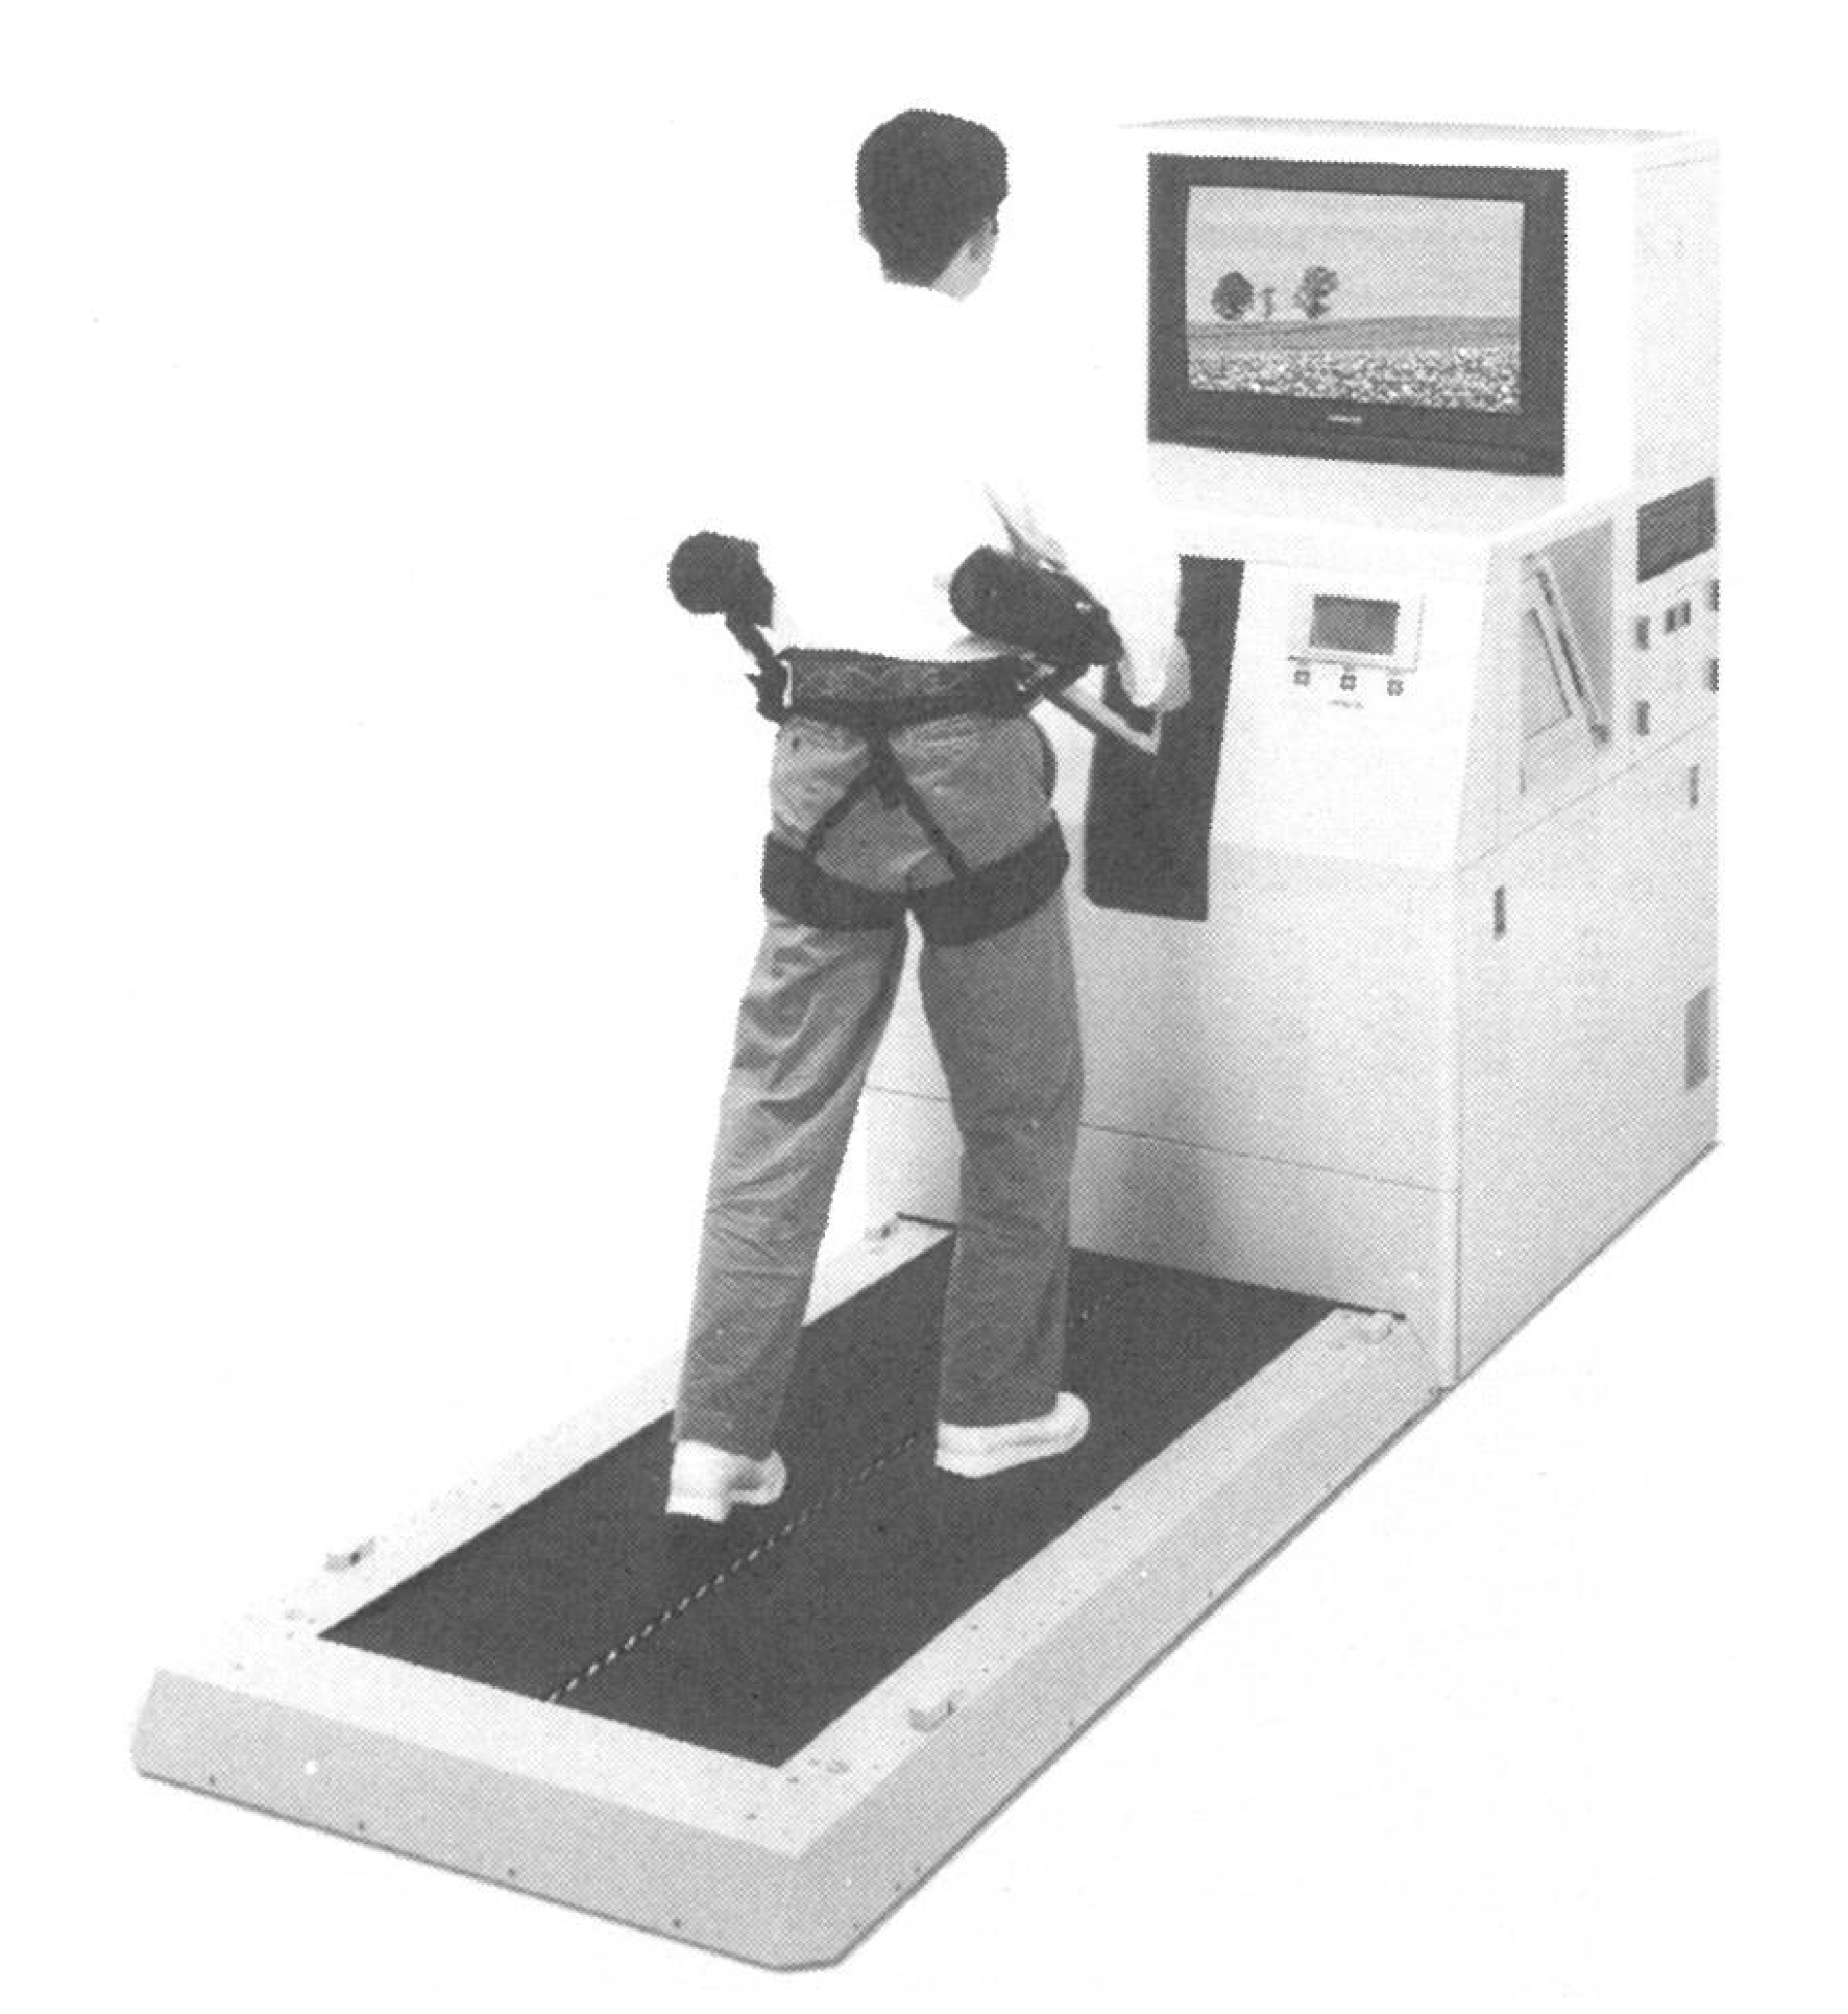
\includegraphics[width=0.5\textwidth]{chap1-figure/VRhokou.eps}
	\caption{バーチャルリアリティを活用した歩行訓練機器(文献\cite{日立}より引用)}
	\label{fig:hitachi}
\end{figure}

歩行感覚提示に使用するディスプレイの印象評価\cite{ディスプレイの違い}が小林らによって報告されている.ロコモーション・インターフェース\cite{ロコモーション}(LI: Locomotion Interface)を提示するディスプレイとして,プラズマディスプレイとHMDとスクリーンの3タイプのディスプレイを用い,ユーザに与える感覚を測定し分析が行われている.ロコモーション・インターフェースとは,VRにおいて,あたかも現実で歩いているような感覚を体感できる装置である.小林らの調査の結果,ディスプレイの違いによってユーザの感覚に差は僅差であったと報告されている.そのことから,ベッド型の下肢リハビリ装置には,着脱可能なHMDの利用が容易であると考えられる.

いずれの関連研究も自立で立ち上がることが可能なリハビリ患者を対象としており,寝たきりの患者は対象とされていない.
そこで本研究では,寝たきりの患者も対象とし,下肢リハビリを行う際の退屈さや歩行の想像の助けを行うシステムの開発をする.
\fi

\section{本研究の目的}
本研究では,ICTを使用し,運動教室で実施される集団でのコグニサイズにおいて,認知課題の負荷を個別に調整する支援を行うことを目的とする.認知課題の正答率を蓄積し,蓄積した認知課題の正答率に応じて,認知課題の負荷を調整可能なシステムを開発する.運動教室の参加者が提案システムを使用することによって,個別に認知症予防の効果があるコグニサイズを実施できることが期待される.また,認知課題の視覚的フィードバックを行うことで,参加者のモチベーションの向上が期待される.

\section{論文の構成}
本稿の構成について述べる.第2章では提案システムの概要と処理の流れについて述べ,第3章では,提案システムを用いた実験および実験の考察について述べる.第4章では,以上で述べたことをまとめ,今後の課題について述べる.

\if0
本稿の構成について述べる.第2章では提案システムの概要と処理の流れについて述べ,第3章では,提案システムに関するSD法を使用したアンケートと記述式のアンケートで印象の評価を行う.そして,評価の結果からの考察を述べる.第4章では,以上で述べたことをまとめ,実験の考察の課題に基づき今後の課題を明らかにする.
\fi

% Local Variables: 
% mode: japanese-LaTeX
% TeX-master: "root"
% End: 


\chapter{提案システム}

\thispagestyle{myheadings}

\section{はじめに}
本章では,運動教室で実施される集団でのコグニサイズにおいて,認知課題の負荷を個別に調整可能なシステムを提案する.本稿では,コグニサイズの一つであるコグニステップに対応した提案システムを開発する.提案システムでは,コグニステップの認知課題の正答率を蓄積し,蓄積した認知課題の正答率に応じて認知課題の負荷を個別に調整する.また,参加者に対して認知課題の視覚的フィードバックを行う.

\if0
本章では,ベッド型の下肢リハビリを拡張する,下肢リハビリへのモチベーションを向上させるための没入型歩行感覚提示システムについて述べる.提案システムは没入感が高を高めるため,現実的な3DCGを利用し実現する.センサが内蔵されたHMDを使用することで,リハビリ患者の頭部の動きに追従した映像提示により,没入感が高まることが期待できる.
\fi

\subsection{コグニステップ}
1.1節で示したとおり,コグニステップは数字を数えながら左右の足で交互にステップをする運動と同時に,一定間隔ごとの決められた数字で拍手をする認知課題を行う.文献\cite{認知症予防へ向けた運動コグニサイズ}では,拍手をする数字の間隔を変更することで認知課題の負荷を調整可能としている.次節以降に提案システムの概要,処理の流れについて述べる.

\section{提案システムの概要}
提案システムでは,身体動作の認識が可能なKinectを使用し,認知課題の拍手動作を検出する.検出した拍手動作を利用し,認知課題の正誤判定を行う.認知課題の正誤判定をコグニステップ実施中に集計し,コグニステップ終了後に集計結果から認知課題の正答率を算出する.算出した認知課題の正答率はデータベースに蓄積する.提案システムの構成図を図\ref{fig:system}に示す.認知課題の視覚的フィードバックを行うために,Kinectに内蔵されるRGBカメラで参加者を撮影し,撮影した動画を参加者の正面にプロジェクタで投影する.プロジェクタ投影面には図\ref{fig:projection_surface}で示すように,認知課題を個別に表示する.表示する認知課題はPC上の管理画面で個別に変更可能である.図\ref{fig:system_management}にPC上の管理画面を示す.データベースに蓄積した認知課題の正答率を図\ref{fig:check_answer_rate}で示すPC上の管理画面で参照し,認知課題の正答率に応じて認知課題を個別に変更する.参加者がプロジェクタ投影面に表示される認知課題のコグニステップを実施することで,認知課題の負荷を個別に調整する支援とする.次節以降に提案システムの処理について述べる.


\begin{figure}[tbp]
	\centering
			\includegraphics[width=0.9\textwidth]{chap2-figure/system.eps}
	\caption{システム構成図}
	\label{fig:system}
\end{figure}

\if0
\begin{figure}[tbp]
	\centering
			\includegraphics[width=0.6\textwidth]{chap2-figure/kinect.eps}
	\caption{Kinect}
	\label{fig:kinect}
\end{figure}
\fi

\begin{figure}[tbp]
	\centering
			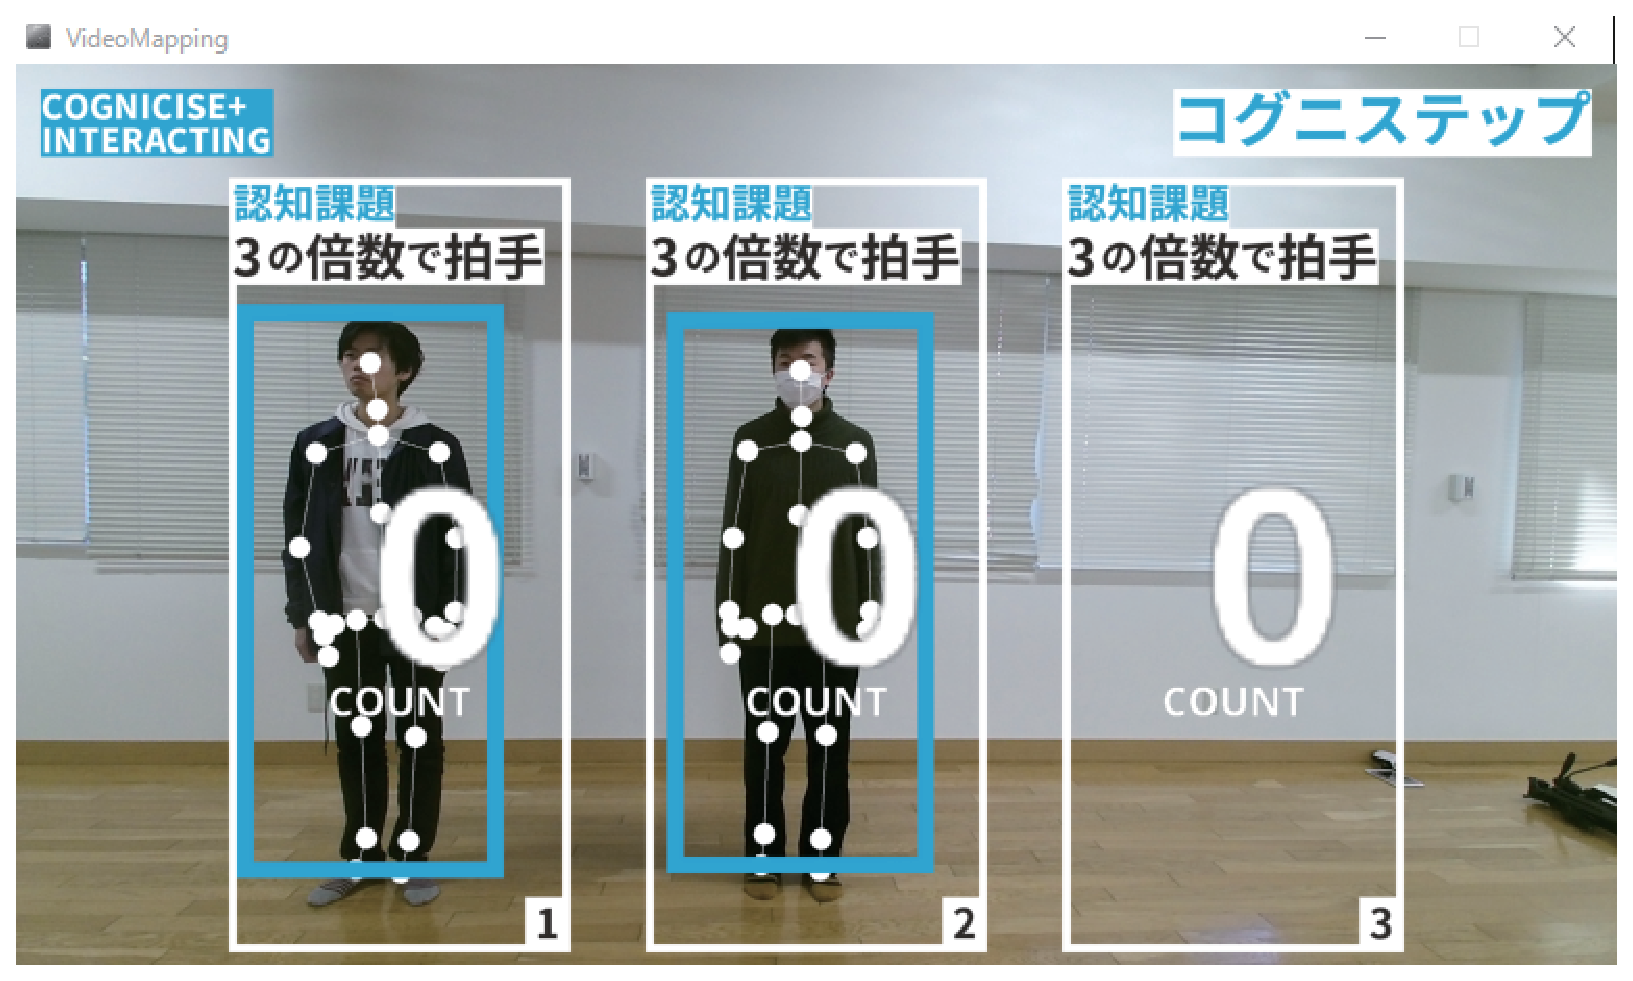
\includegraphics[width=0.9\textwidth]{chap2-figure/vm_init.eps}
	\caption{プロジェクタ投影面(赤枠内が認知課題)}
	\label{fig:projection_surface}
\end{figure}

\begin{figure}[tbp]
	\centering
			\includegraphics[width=0.9\textwidth]{chap2-figure/db_init.eps}
	\caption{PC上のシステムの管理画面}
	\label{fig:system_management}
\end{figure}

\begin{figure}[tbp]
	\centering
			\includegraphics[width=0.9\textwidth]{chap2-figure/db_user_info.eps}
	\caption{PC上のシステムの管理画面(赤枠内が認知課題の正答率)}
	\label{fig:check_answer_rate}
\end{figure}


\if0
提案システムでは,ベッド型の下肢リハビリ装置の下肢可動部にKinectV2\cite{KinectV2}を置き,歩行の検出を行う.KinectV2を図\ref{fig:kinect}に示す.KinectV2をセンサとして使用する.提案システムの歩行の検出にKinectV2を使用したシステム構成を図\ref{fig:beforesystemarc}に示す.ベッド型の下肢リハビリ装置の下肢部分の手前にKinectV2を設置する.処理の流れを図\ref{fig:片桐1}に示す.KinectV2からの取得した映像を二値化行い,図\ref{fig:kinectsystemarc}に示す,ベッド型の下肢リハビリ装置の下肢可動部の検出を行う.図\ref{fig:kinectsystemarc}に示す矩形の重心点の座標を取得し閾値を設定し,歩行判定を行う.歩行判定を基にキャラクタは歩行動作を行う.

\begin{figure}[tbp]
	\centering
			\includegraphics[width=0.8\textwidth,angle = 270]{chap2-figure/kinect.eps}
	\caption{KinectV2}
	\label{fig:kinect}
\end{figure}

\begin{figure}[tbp]
	\centering
			\includegraphics[width=0.8\textwidth]{chap2-figure/beforesystem.eps}
	\caption{KinectV2を使用したシステム構成図}
	\label{fig:beforesystemarc}
\end{figure}

\begin{figure}[tbp]
	\centering
			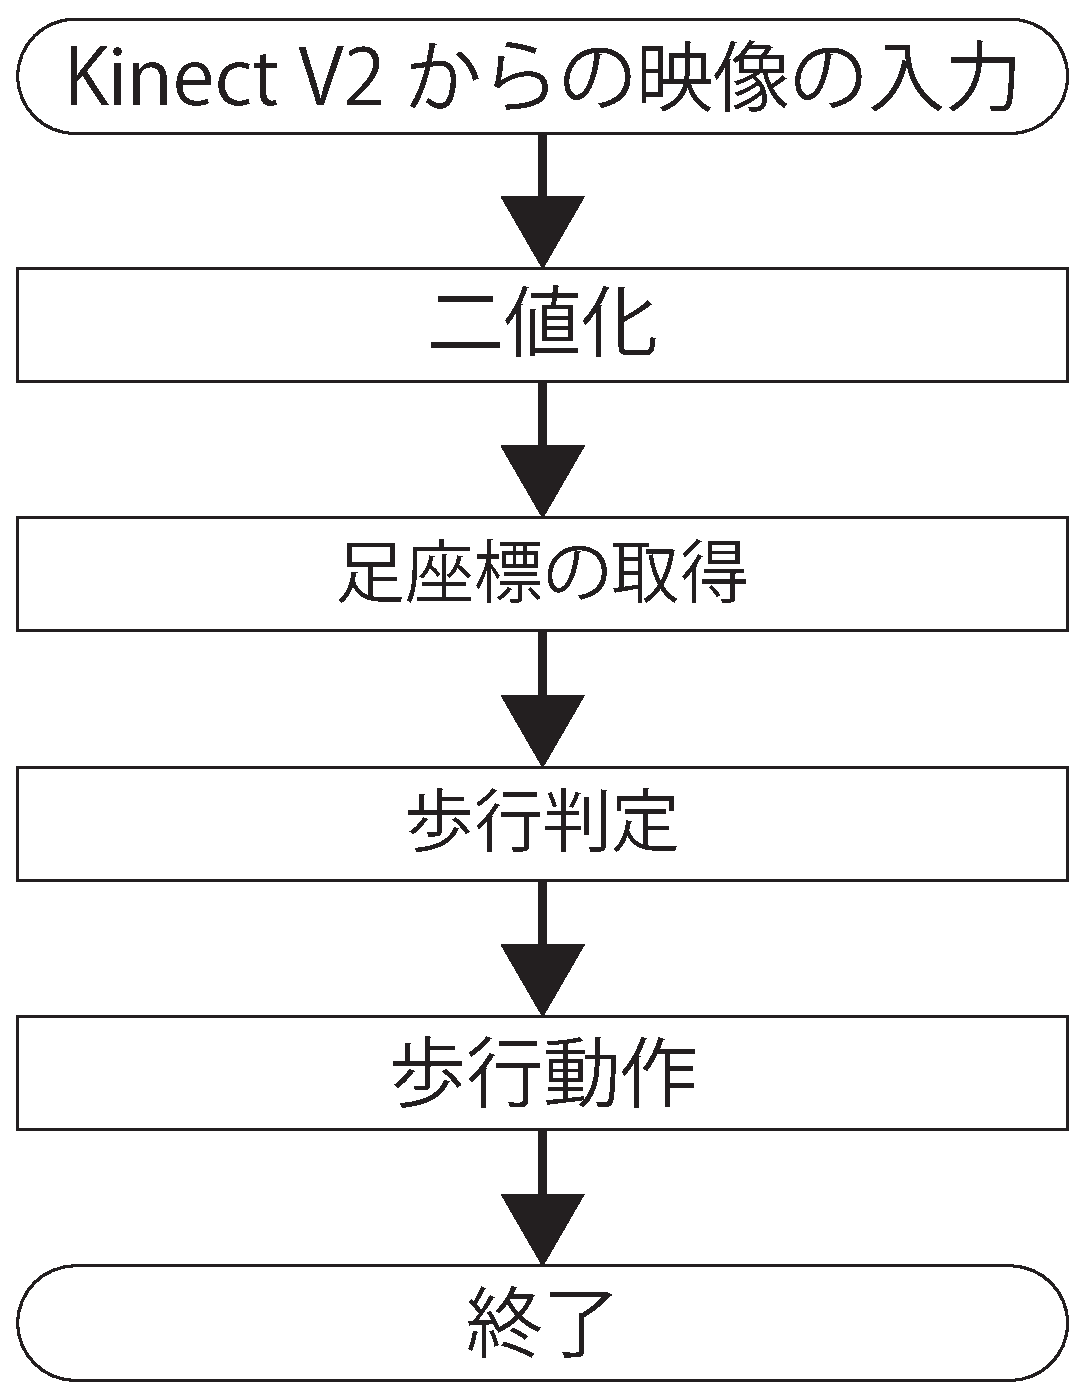
\includegraphics[width=0.3\textwidth]{chap2-figure/katagiri1.eps}
	\caption{処理の流れ}
	\label{fig:片桐1}
\end{figure}

\begin{figure}[tbp]
	\centering
			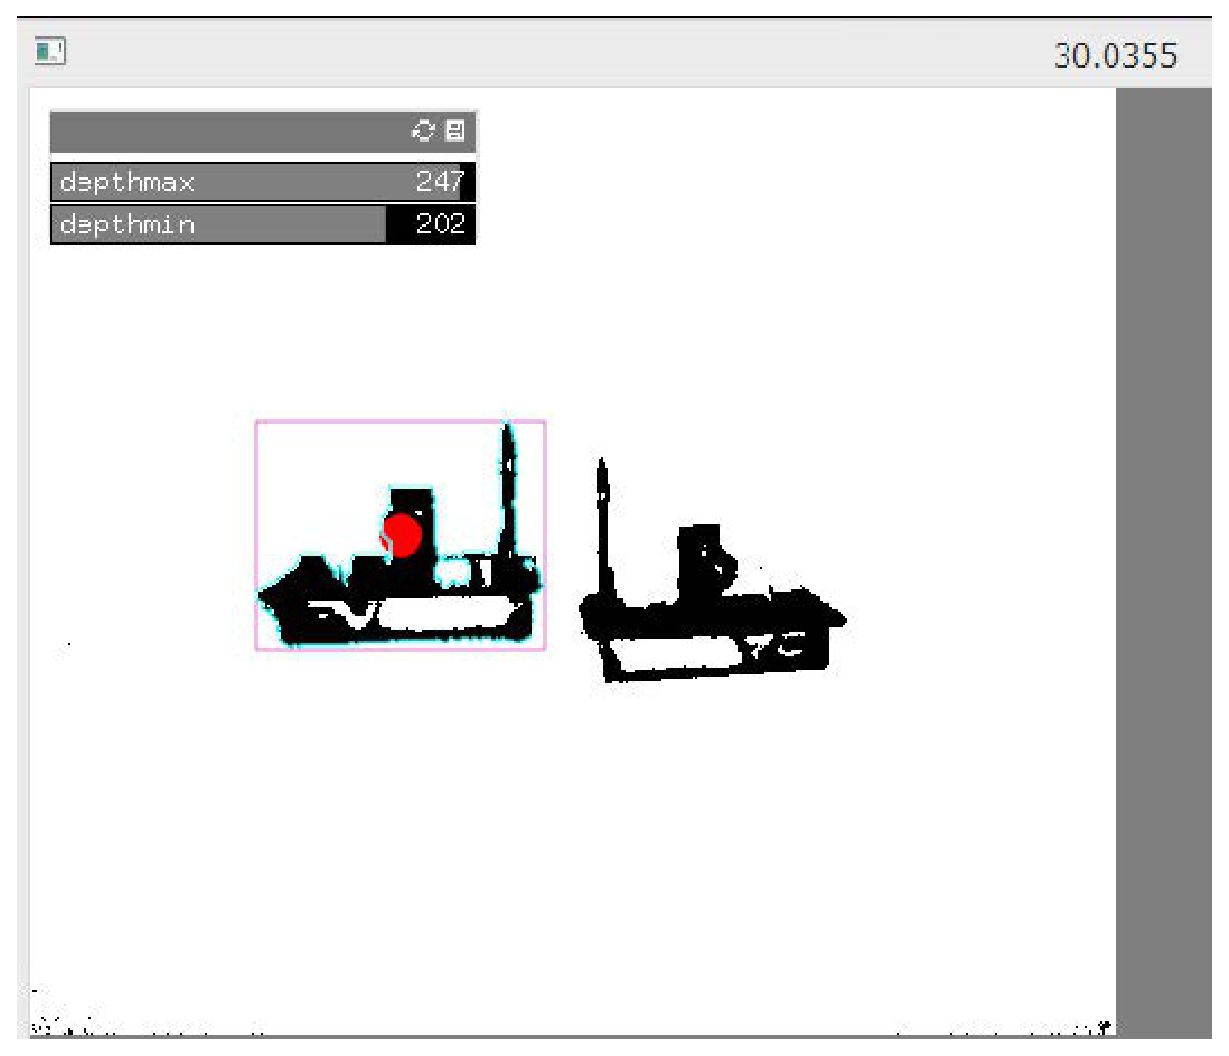
\includegraphics[width=0.8\textwidth]{chap2-figure/kinectsystem.eps}
	\caption{KinectV2の検出画像}
	\label{fig:kinectsystemarc}
\end{figure}
\fi

\section{処理の流れ}
提案システムの処理の流れについて述べる.提案システムの処理の流れは,参加者が初めて提案システムを使用する場合と,二回目以降に使用する場合で異なる.

\subsection{参加者が初めて提案システムを使用する場合}
参加者が初めて提案システムを使用する場合の処理の流れを述べる.

\subsection{参加者が二回目以降に提案システムを使用する場合}
参加者が二回目以降に提案システムを使用する場合の処理の流れを述べる.


\if0
提案システムの処理の流れについて述べる.処理の流れを図\ref{fig:片桐2}に示す.
提案システムの開始方法は,HMDをつなげたPCのマウスを左クリック又はキーボードのスペースキーで開始される.HMDに提示される開始画面を図\ref{fig:start}に示す.開始後,キャラクタの一人称視点の映像が提示され歩行が開始される.開始後の画面を図\ref{fig:gemestart}に示す.患者は設定時間が終了するまで下肢リハビリを続ける.設定した時間が終了すると,図\ref{fig:end}の画面が提示される.
\fi

\begin{figure}[tbp]
	\centering
			\includegraphics[width=0.9\textwidth]{chap2-figure/db_management_user.eps}
	\caption{参加者の管理画面}
	\label{fig:db_management_user}
\end{figure}

\begin{figure}[tbp]
	\centering
			\includegraphics[width=0.9\textwidth]{chap2-figure/db_regist_new_user.eps}
	\caption{新規参加者の登録画面}
	\label{fig:db_regist_new_user}
\end{figure}

\begin{figure}[tbp]
	\centering
			\includegraphics[width=0.9\textwidth]{chap2-figure/db_select_user.eps}
	\caption{参加者の選択画面}
	\label{fig:db_select_user}
\end{figure}

\begin{figure}[tbp]
	\centering
			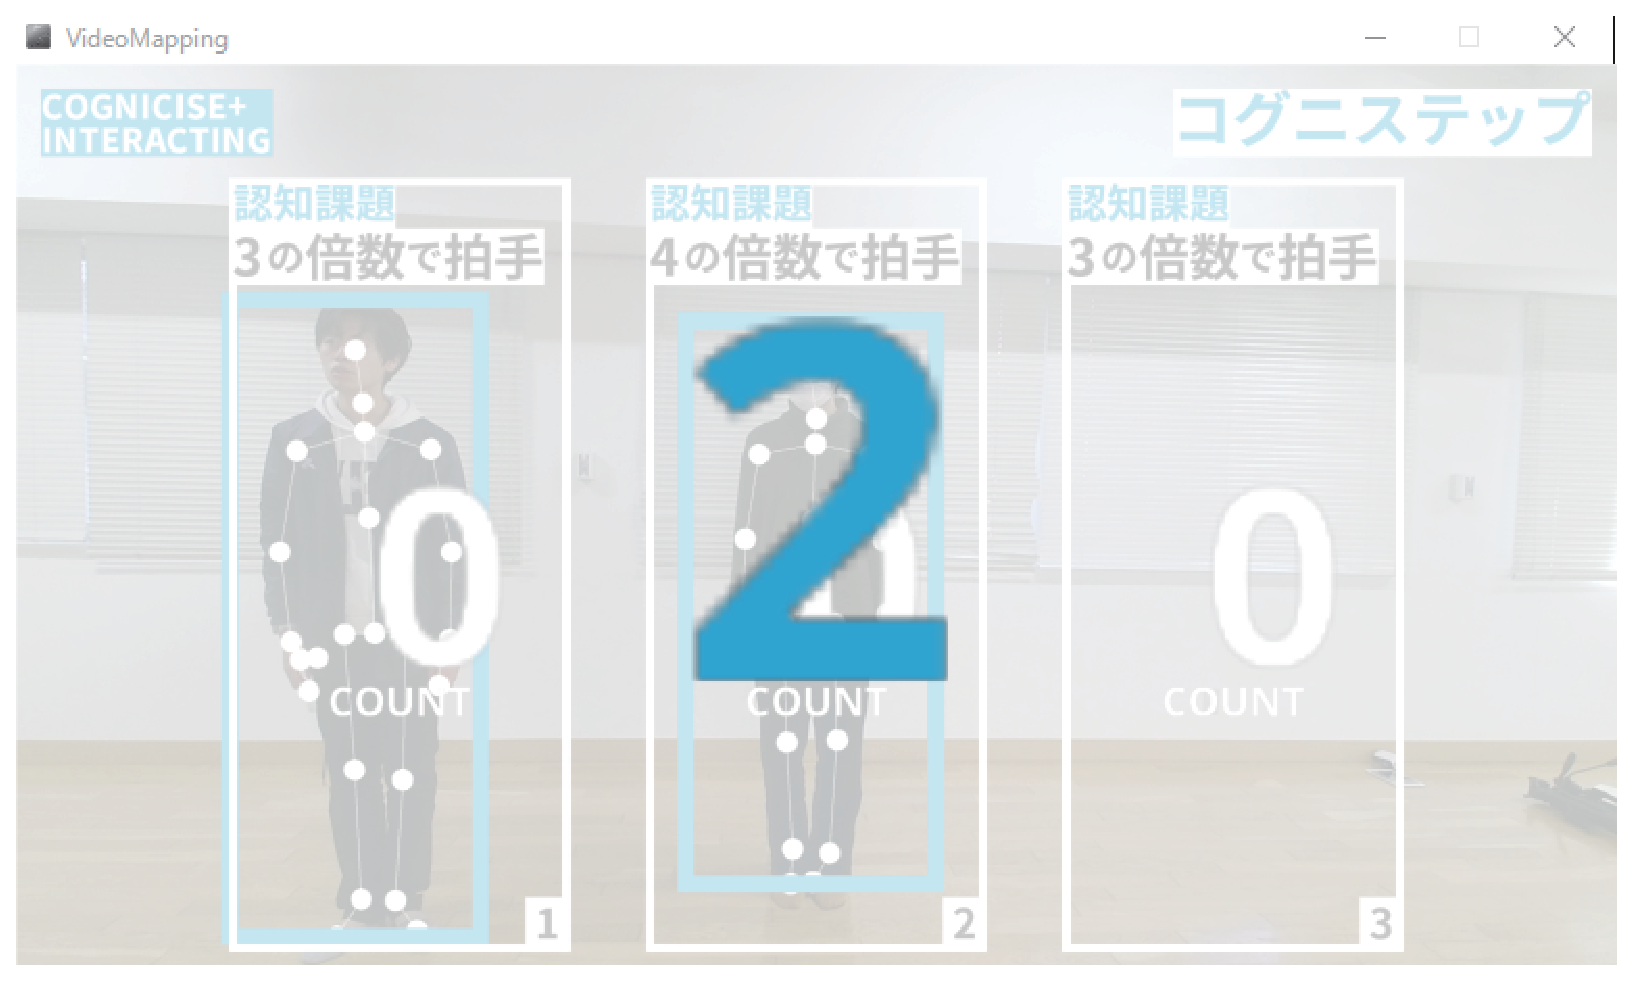
\includegraphics[width=0.9\textwidth]{chap2-figure/vm_start.eps}
	\caption{プロジェクタ投影面(開始時)}
	\label{fig:vm_start}
\end{figure}

\begin{figure}[tbp]
	\centering
			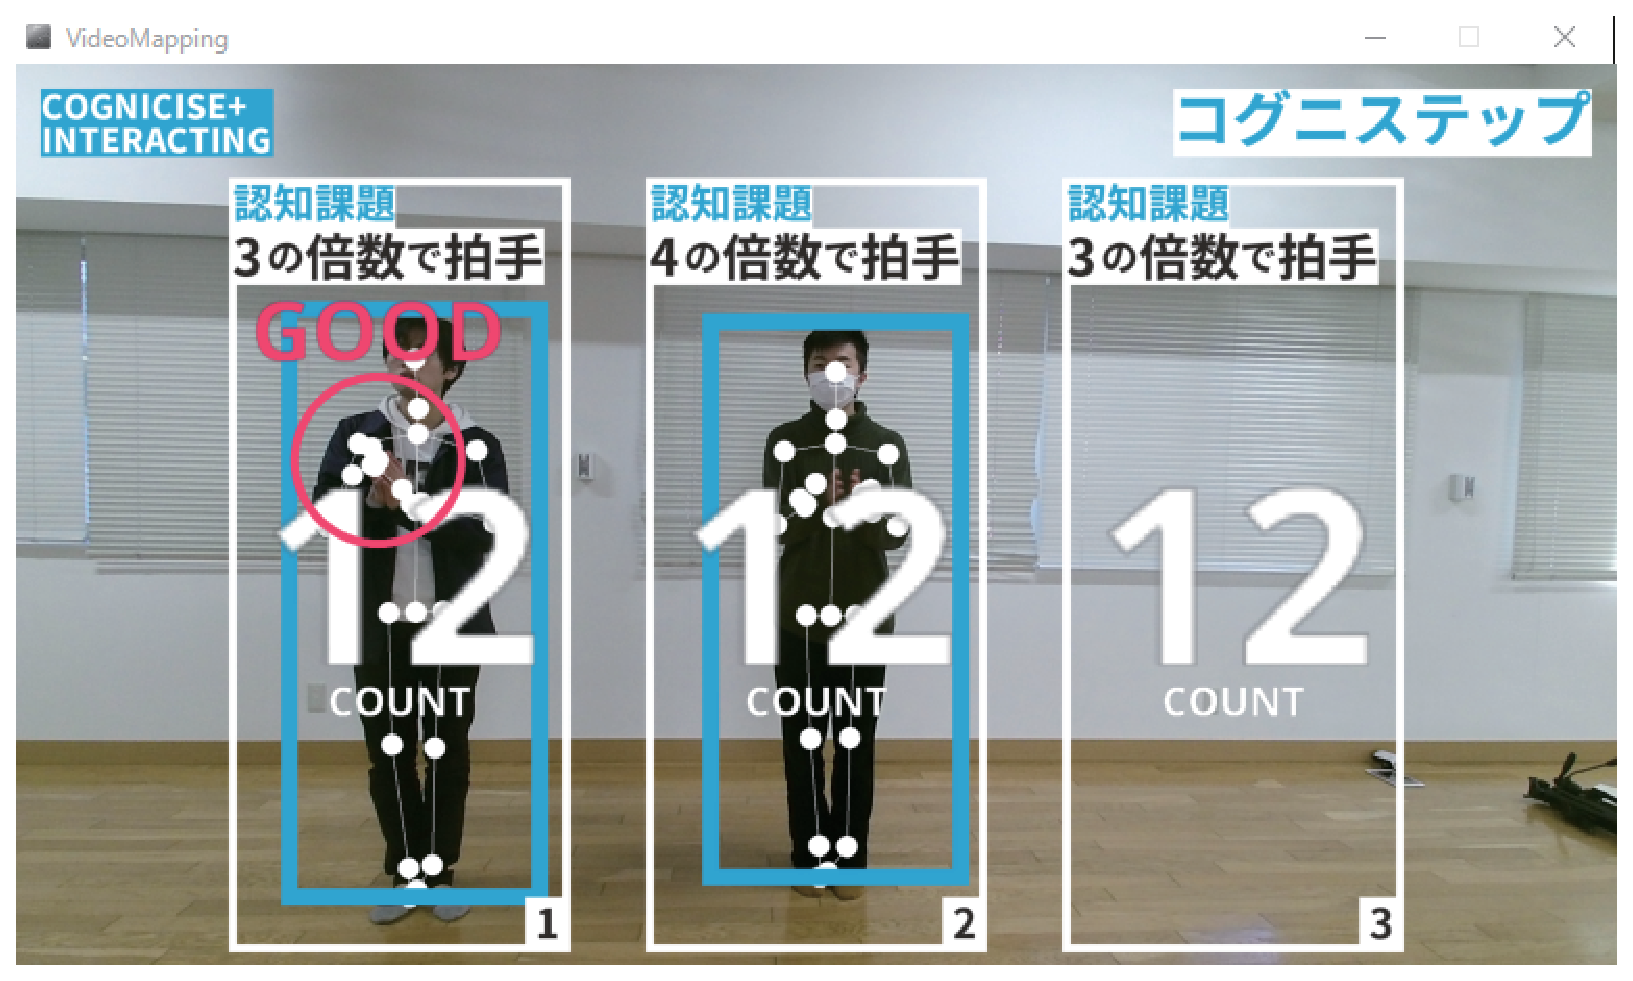
\includegraphics[width=0.9\textwidth]{chap2-figure/vm_clap.eps}
	\caption{プロジェクタ投影面(認知課題の正答時)}
	\label{fig:vm_clap}
\end{figure}

\begin{figure}[tbp]
	\centering
			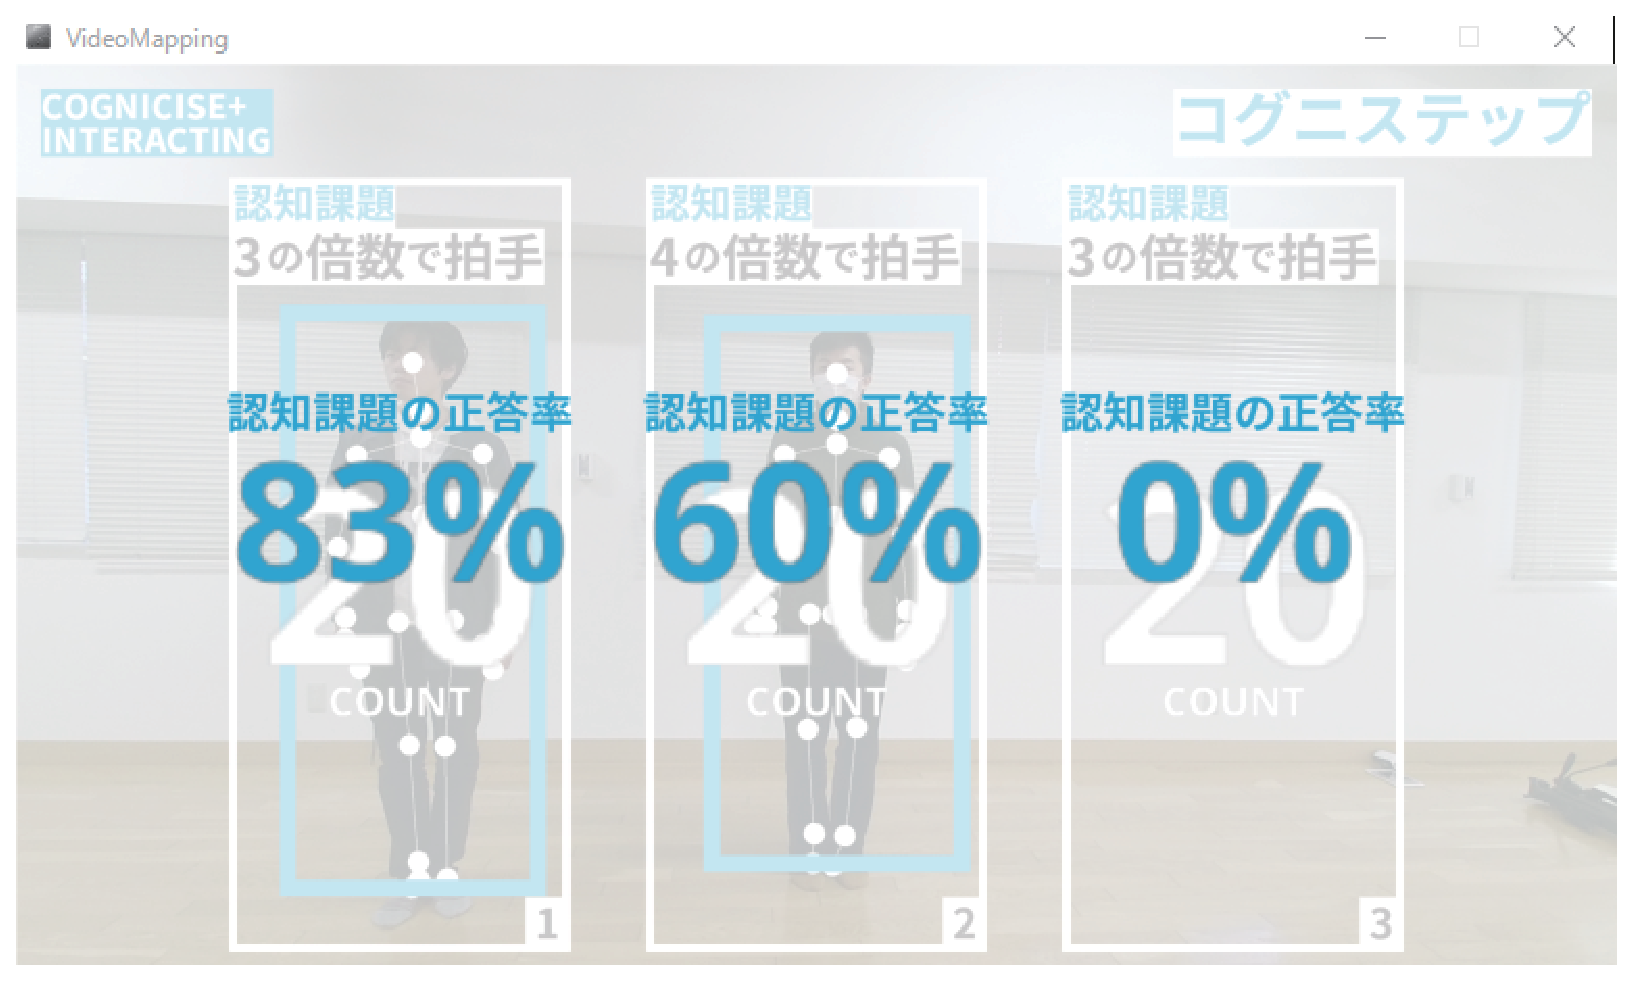
\includegraphics[width=0.9\textwidth]{chap2-figure/vm_answer_rate.eps}
	\caption{プロジェクタ投影面(認知課題の正答率の表示)}
	\label{fig:vm_answer_rate}
\end{figure}

\begin{figure}[tbp]
	\centering
			\includegraphics[width=0.9\textwidth]{chap2-figure/db_user_info.eps}
	\caption{参加者情報画面}
	\label{fig:db_user_info}
\end{figure}

\begin{figure}[tbp]
	\centering
			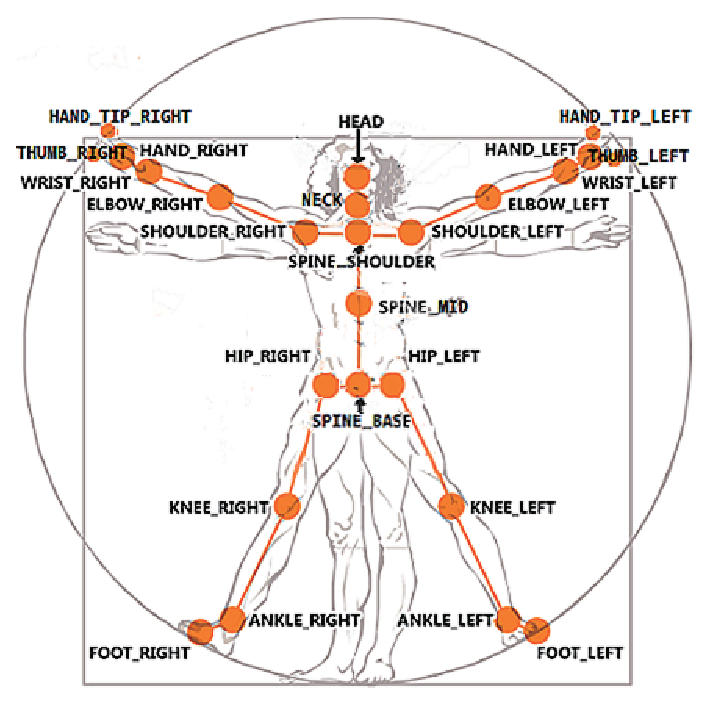
\includegraphics[width=0.7\textwidth]{chap2-figure/skelton_position.eps}
	\caption{Skeleton positions relative to the human body}
	\label{fig:skelton_position}
\end{figure}

\if0
\begin{figure}[tbp]
	\centering
			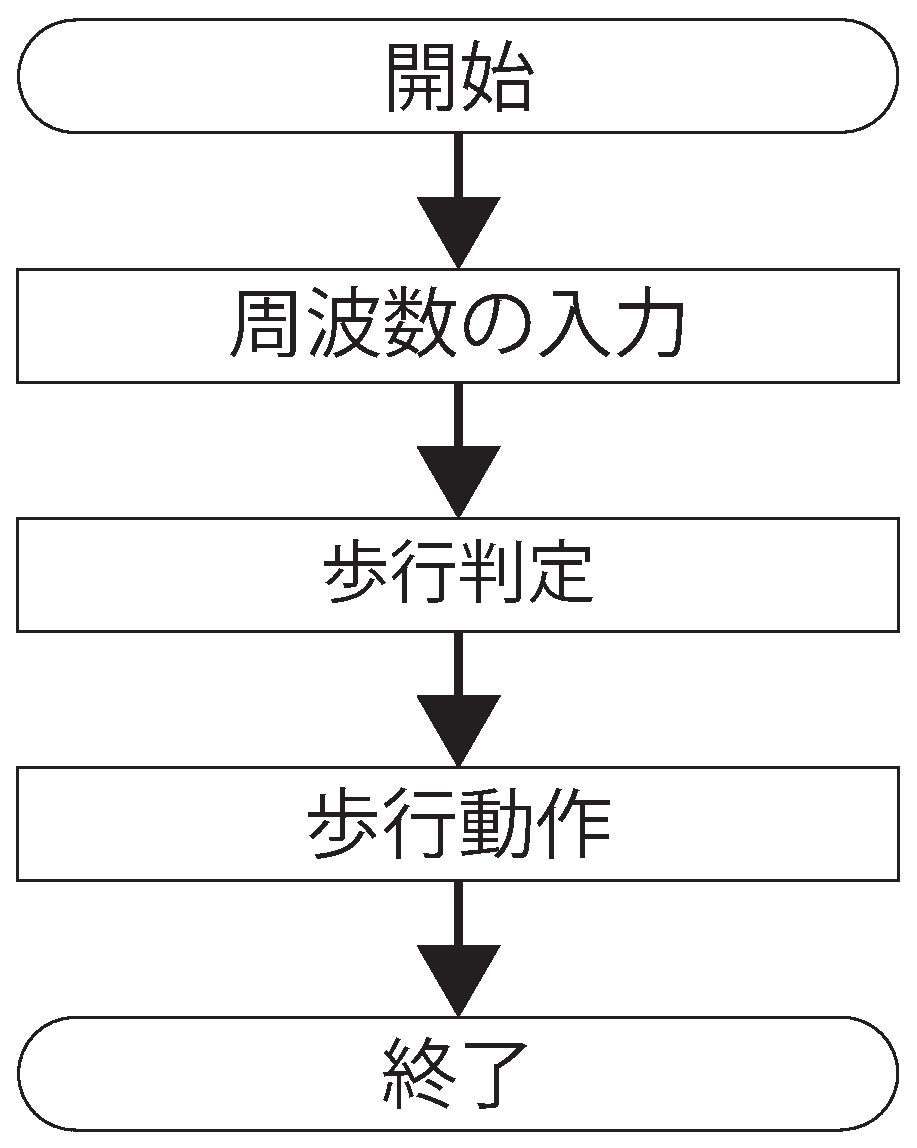
\includegraphics[width=0.3\textwidth]{chap2-figure/katagiri2.eps}
	\caption{処理の流れ}
	\label{fig:片桐2}
\end{figure}

\begin{figure}[tbp]
	\centering
			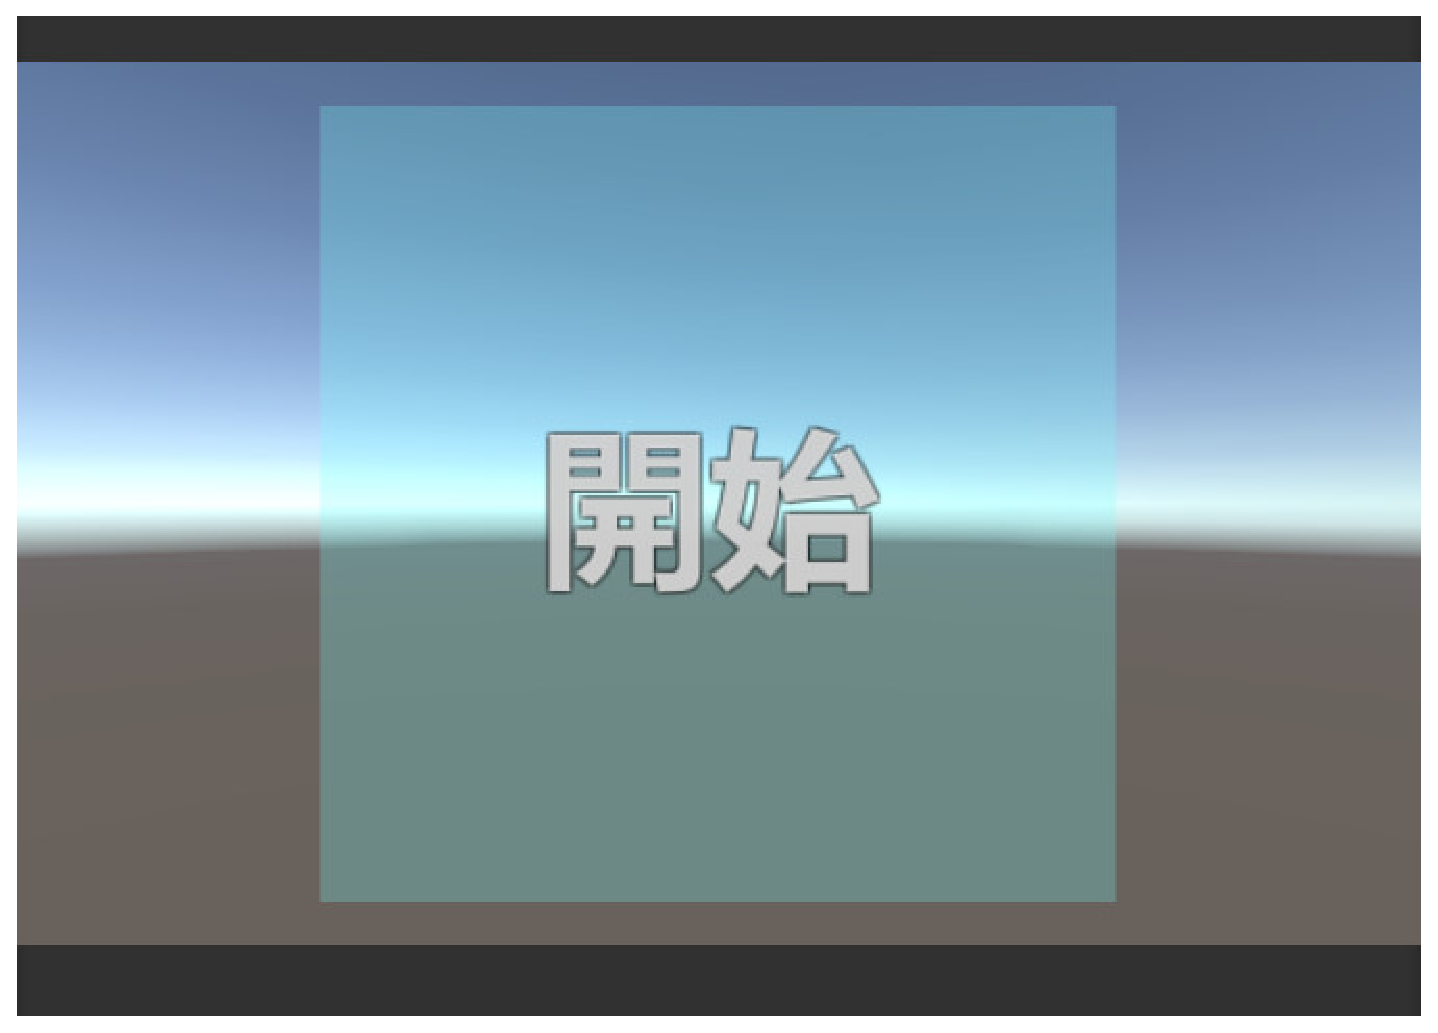
\includegraphics[width=0.9\textwidth]{chap2-figure/start.eps}
	\caption{スタート画面}
	\label{fig:start}
\end{figure}

\begin{figure}[tbp]
	\centering
			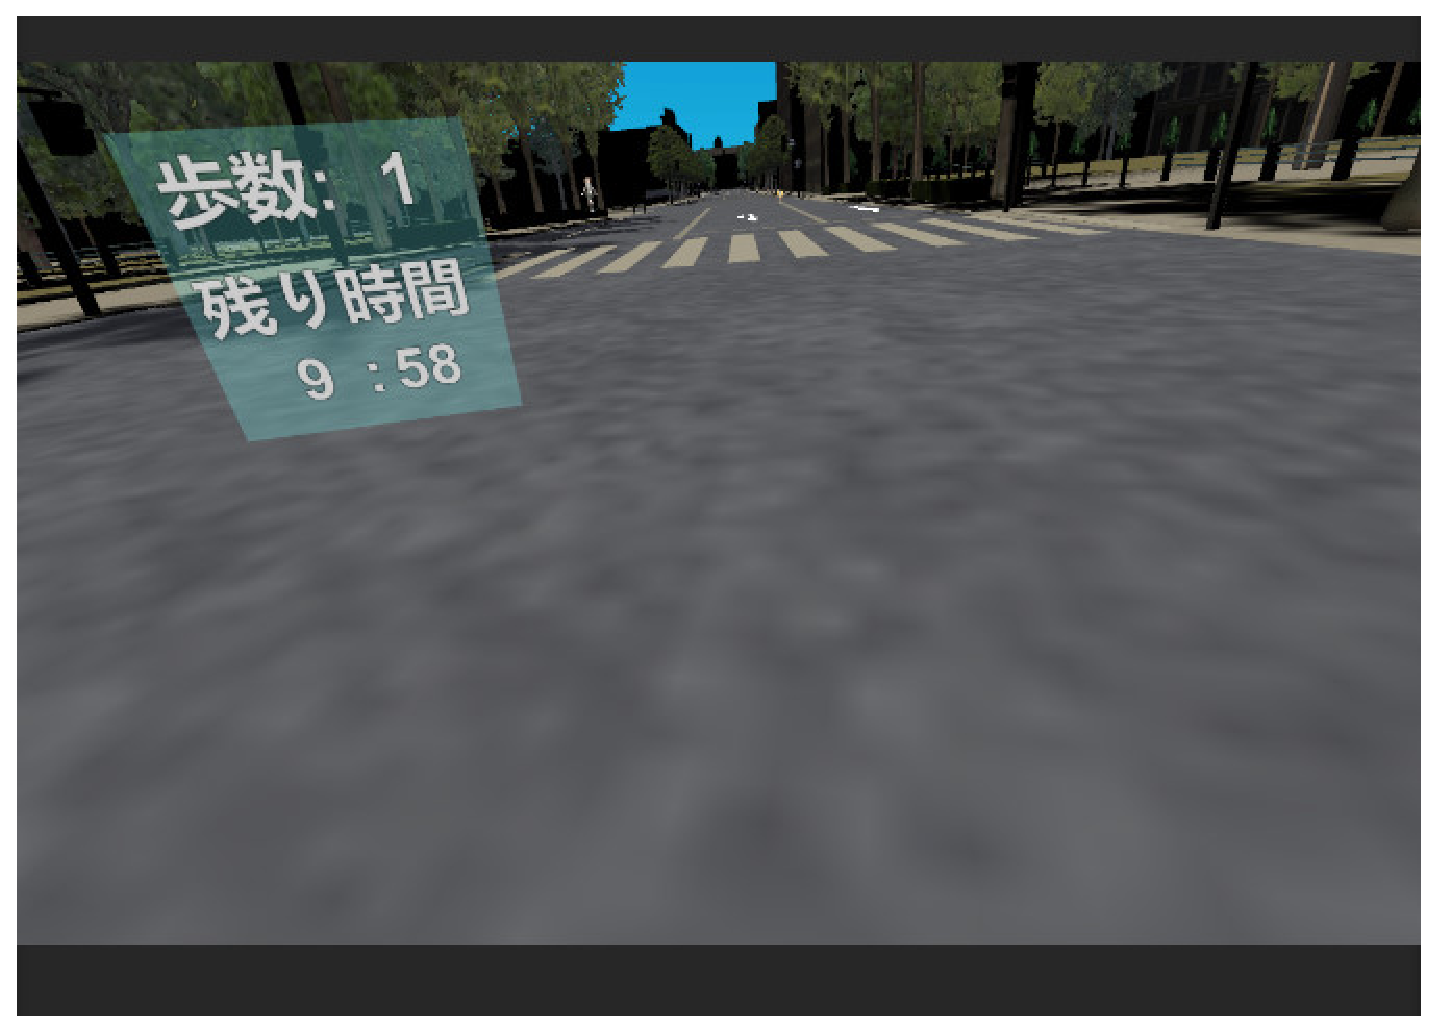
\includegraphics[width=0.9\textwidth]{chap2-figure/midstream-1.eps}
	\caption{開始後画面}
	\label{fig:gemestart}
\end{figure}

\begin{figure}[tbp]
	\centering
			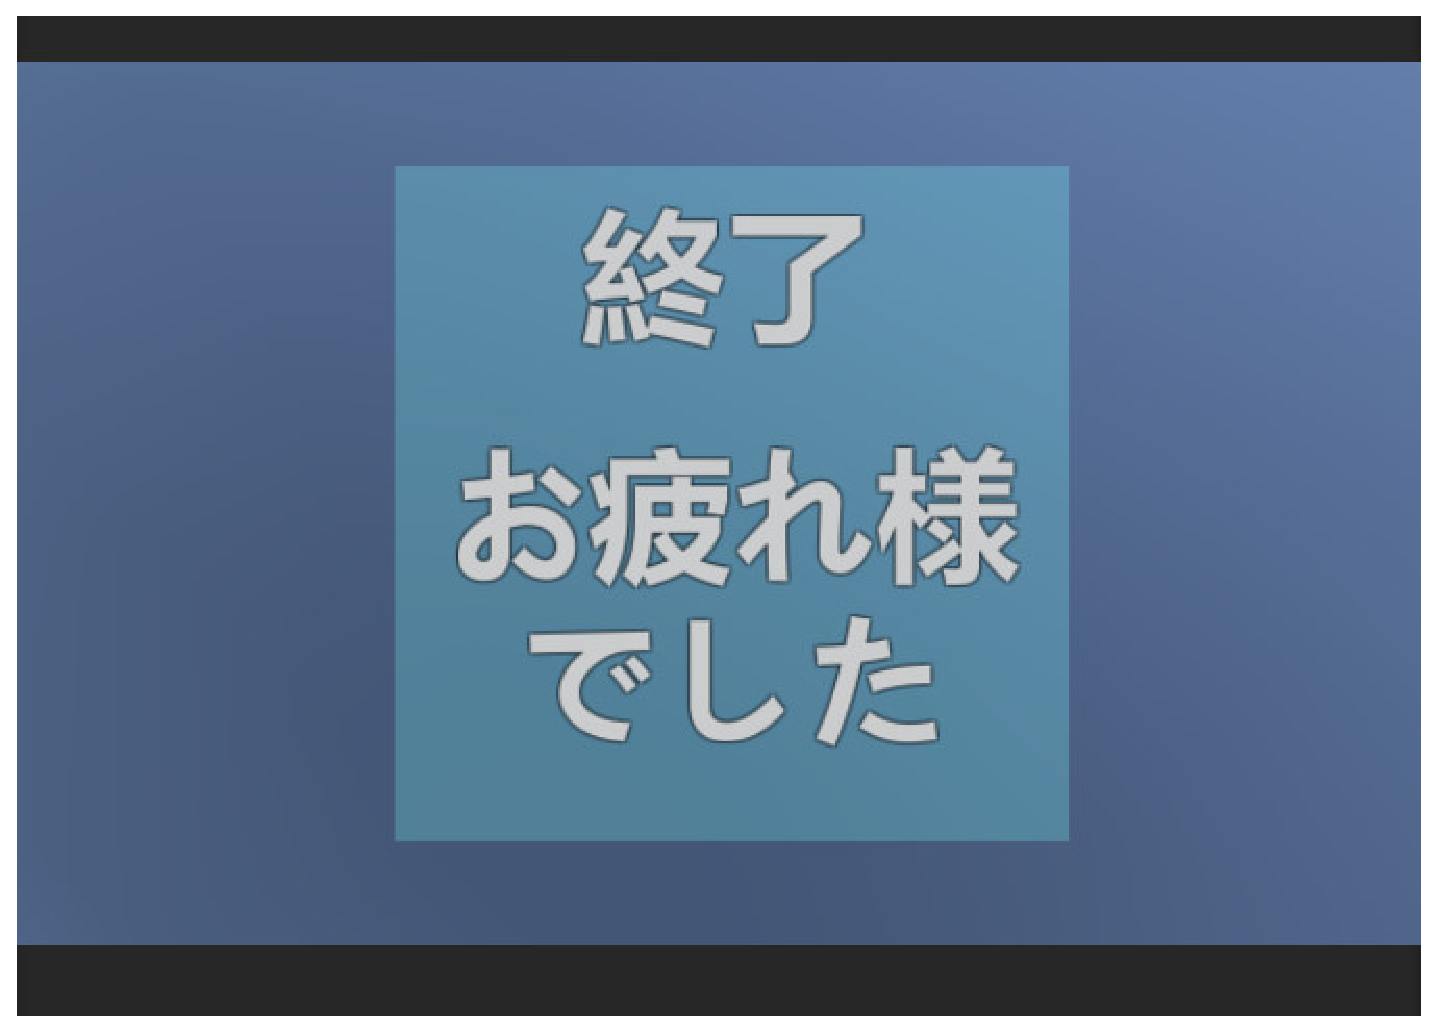
\includegraphics[width=0.9\textwidth]{chap2-figure/end.eps}
	\caption{終了画面}
	\label{fig:end}
\end{figure}
\fi

\if0
\subsection{歩行距離の設定}
CGキャラクタの歩行距離は,ベッド型の下肢リハビリ装置から読み取れる動作周波数から計算され,動作周波数$N$秒間の1周期ごとに,CGキャラクタが$M$m進む.設定した時間までCGキャラクタは歩行動作を続ける.

\subsection{キャラクタの視点設定}
HMDには,センサが内蔵されており,頭部の動きに応じて映像がリアルタイムに追従するので,仮想空間に没入できる利点がある.すなわち,患者が頭部を動かすと,仮想空間内に配置されたCGキャラクタの視点も追従して変わり,HMDの持つ没入感という利点を活かしている.図\ref{fig:geammidstream}に,プレイ途中に頭部を動かした一例を示す.

\begin{figure}[tbp]
	\centering
			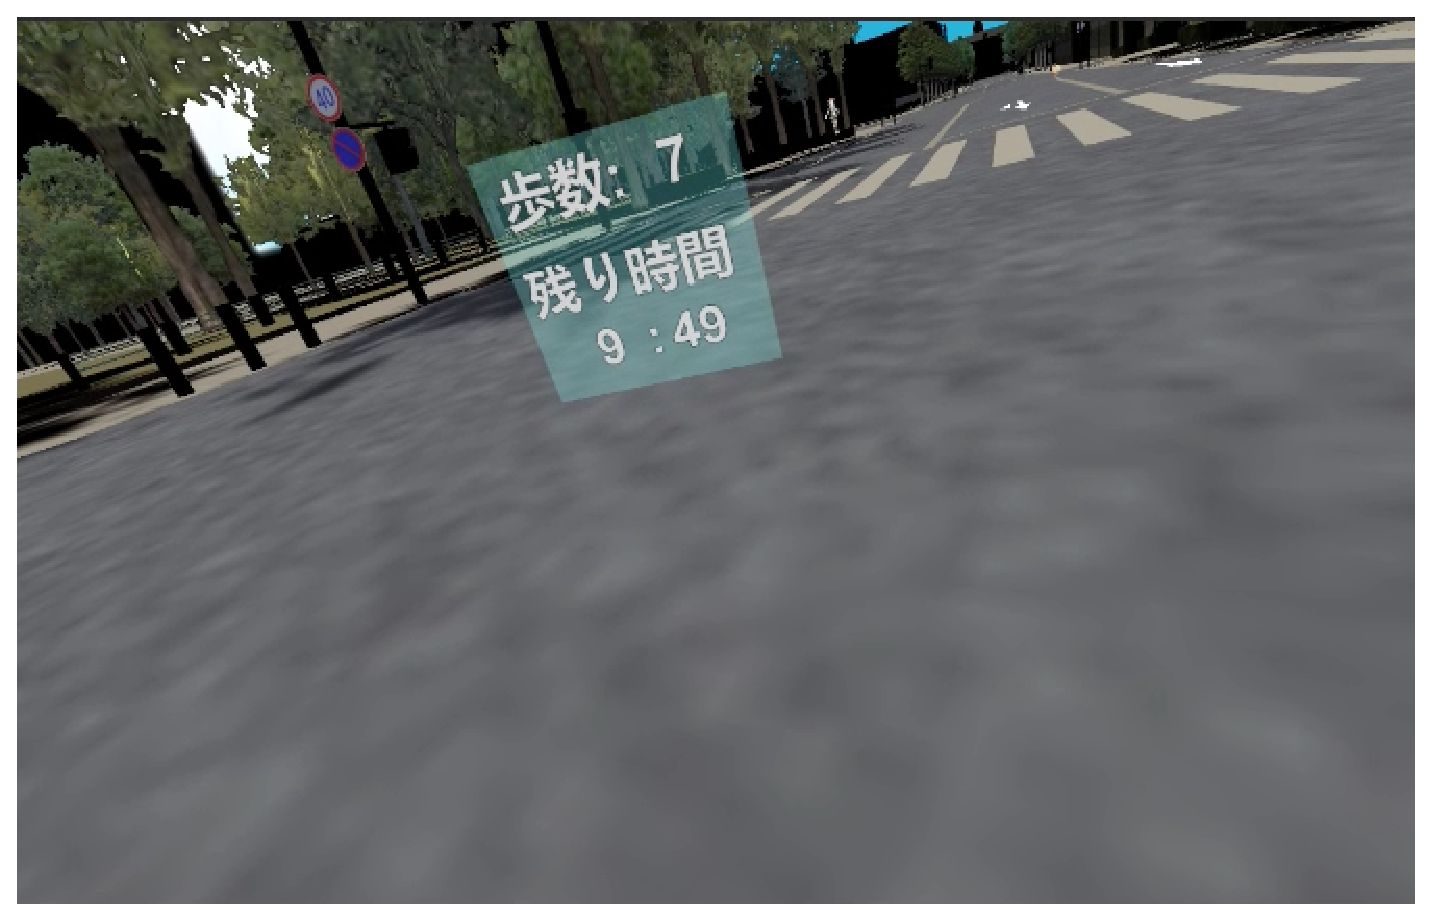
\includegraphics[width=0.9\textwidth]{chap2-figure/midstream-2.eps}
	\caption{プレイ途中視点を変えた図}
	\label{fig:geammidstream}
\end{figure}
\fi

\section{むすび}

\if0
本章では,ベッド型の下肢リハビリ装置から読み取れる動作周波数から計算されるCGキャラクタの歩行距離によって,3D都市モデル空間でのCGキャラクタの移動を行う手法について述べた.ベッド型の他動歩行器と同時に体験するシステムのためのキャラクタの視点の変更を行う手法を記述した.第3章では,大学生の被験者に対して行った提案システムに関するアンケート評価について述べる.
\fi

% Local Variables: 
% mode: japanese-LaTeX
% TeX-master: "root"
% End: 


%\chapter{実験と考察}
\thispagestyle{myheadings}

\section{はじめに}
本章では,提案システムを実装し,大学生の被験者に対してアンケート評価を行う.そして,各実験のアンケート評価の結果から考察について述べる.
アンケート評価にはSD法を使用した.提案システムに対しての心理的尺度を図り,リハビリに対するモチベーションへの影響を考察する.
\section{実験環境}
実験環境を以下に示す.

\begin{itemize}
 \item OS: Windows8.1
 \item CPU: 4.0GHz Intel Corei7-4790k
 \item GPU: 4GB NIVIDA Geforce GTX970
 \item Memory: 8G DDR3-1600×2
\end{itemize}

HMDには,Oculus VR社のOculusRiftDK2\cite{OculusRift}を使用した.開発環境はUnity\cite{Unity}を使用した.開発環境であるUnityで提供されている3D都市モデル空間アセット\cite{3D都市モデル}を仮想空間として使用する.使用キャラクタを図\ref{fig:chara}に示す.下肢リハビリ装置の動作周波数を約1.67 秒の1周期ごととし,CGキャラクタが0.64m進む設定とした.

\begin{figure}[tbp]
	\centering
			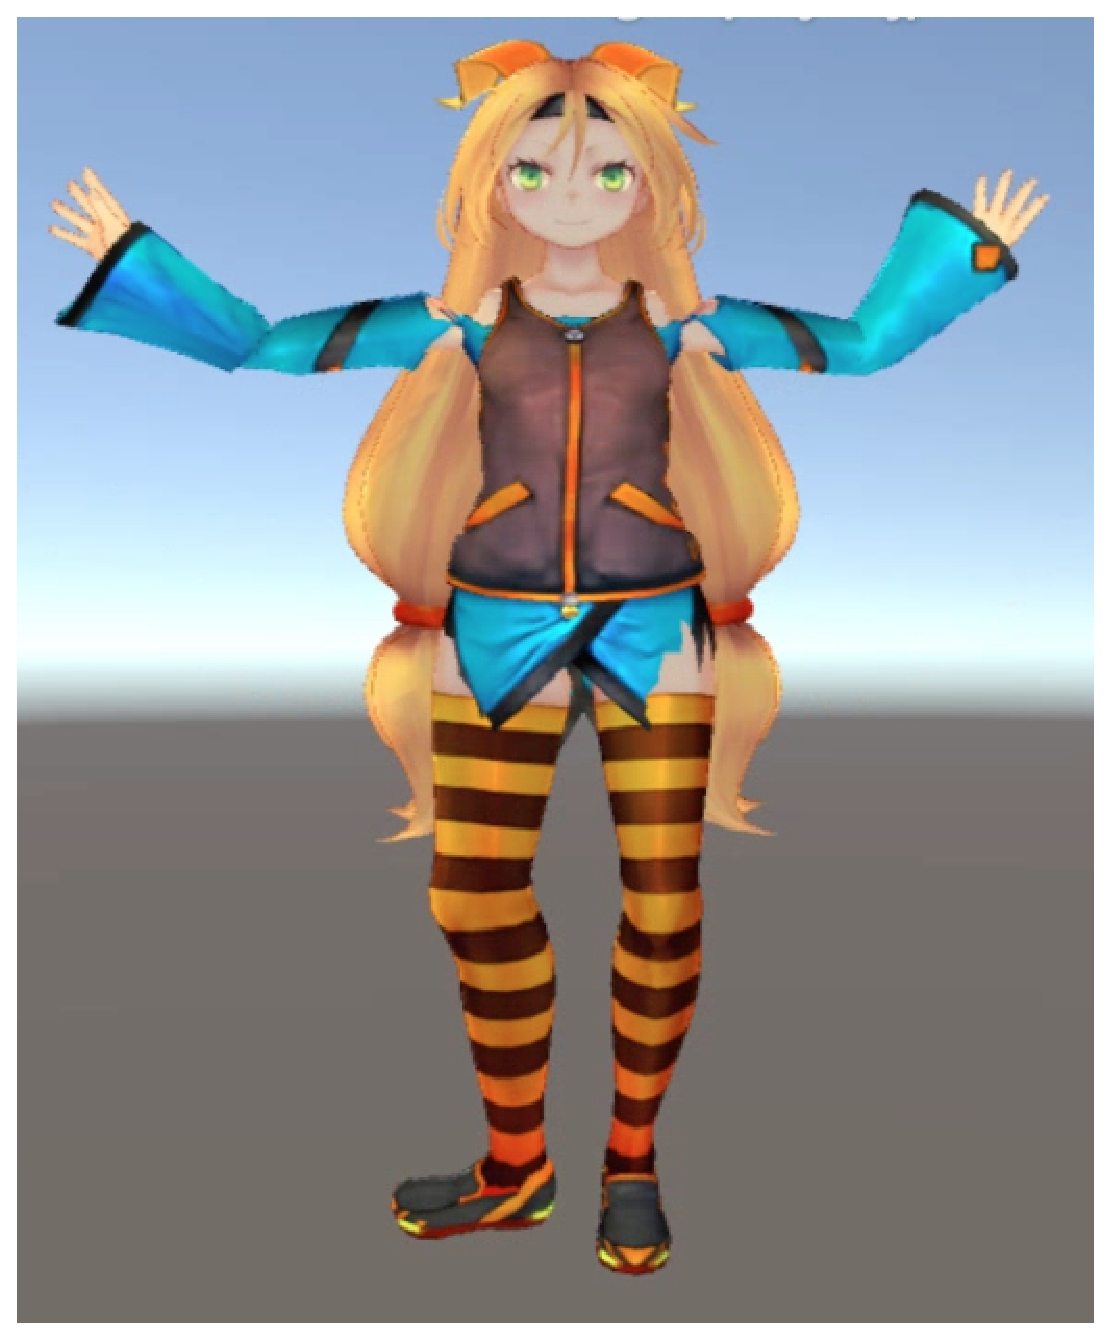
\includegraphics[width=0.5\textwidth]{chap3-figure/UntyChan.eps}
	\caption{使用キャラクタ\protect \footnotemark}
	\label{fig:chara}
\end{figure}
\footnotetext{Unity Technologies Japan/UCL}

\section{使用アンケート}
評価対象は,提案システムを使用した実験(実験1),ベッド型の下肢リハビリ装置のみを使用した実験(実験2),提案システムにおいて風景を変化させない実験(実験3),ベッド型の下肢リハビリ装置を動作させず,HMD の映像のみを視聴した実験(実験4) の4 種類を用意した.10 代から20 代の男性24 名を対象にSD 法の形容詞対と記述式の2種類のアンケートを用いた.使用したアンケートを図\ref{fig:ank1}--\ref{fig:ank4}に示す.実験の体験時間は3 分間である.実験の様子を図\ref{fig:jiken}示す.

\subsection{SD法とは}
SD法\cite{人間工学ガイド}は相反する形容詞対を多数用いて評価することにより,人が「どのように感じるか」といった心理的な印象を明らかにすることができる.今回の実験では,提案システムの絶対的な印象を評価するために,各実験6名ずつに分かれて実験を行った.

\subsection{実験の種類}
評価対象は,提案システムを使用した実験(実験1),ベッド型の下肢リハビリ装置のみを使用した実験(実験2),提案システムにおいて風景を変化させない実験(実験3),ベッド型の下肢リハビリ装置を動作させず,HMD の映像のみを視聴した実験(実験4) の4 種類を用意した.10代から20代の男性24名を対象にSD 法の形容詞対と記述式の2種類のアンケートを用いた.

\begin{figure}[tbp]
	\centering
		\fbox{
			\includegraphics[width=0.9\textwidth]{chap3-figure/a-0.eps}
			}
	\caption{アンケート1枚目}
	\label{fig:ank1}
\end{figure}

\begin{figure}[tbp]
	\centering
		\fbox{
			\includegraphics[width=0.9\textwidth]{chap3-figure/a-1.eps}
		}
	\caption{アンケート2枚目}
	\label{fig:ank2}
\end{figure}
\begin{figure}[tbp]
	\centering
	\fbox{
			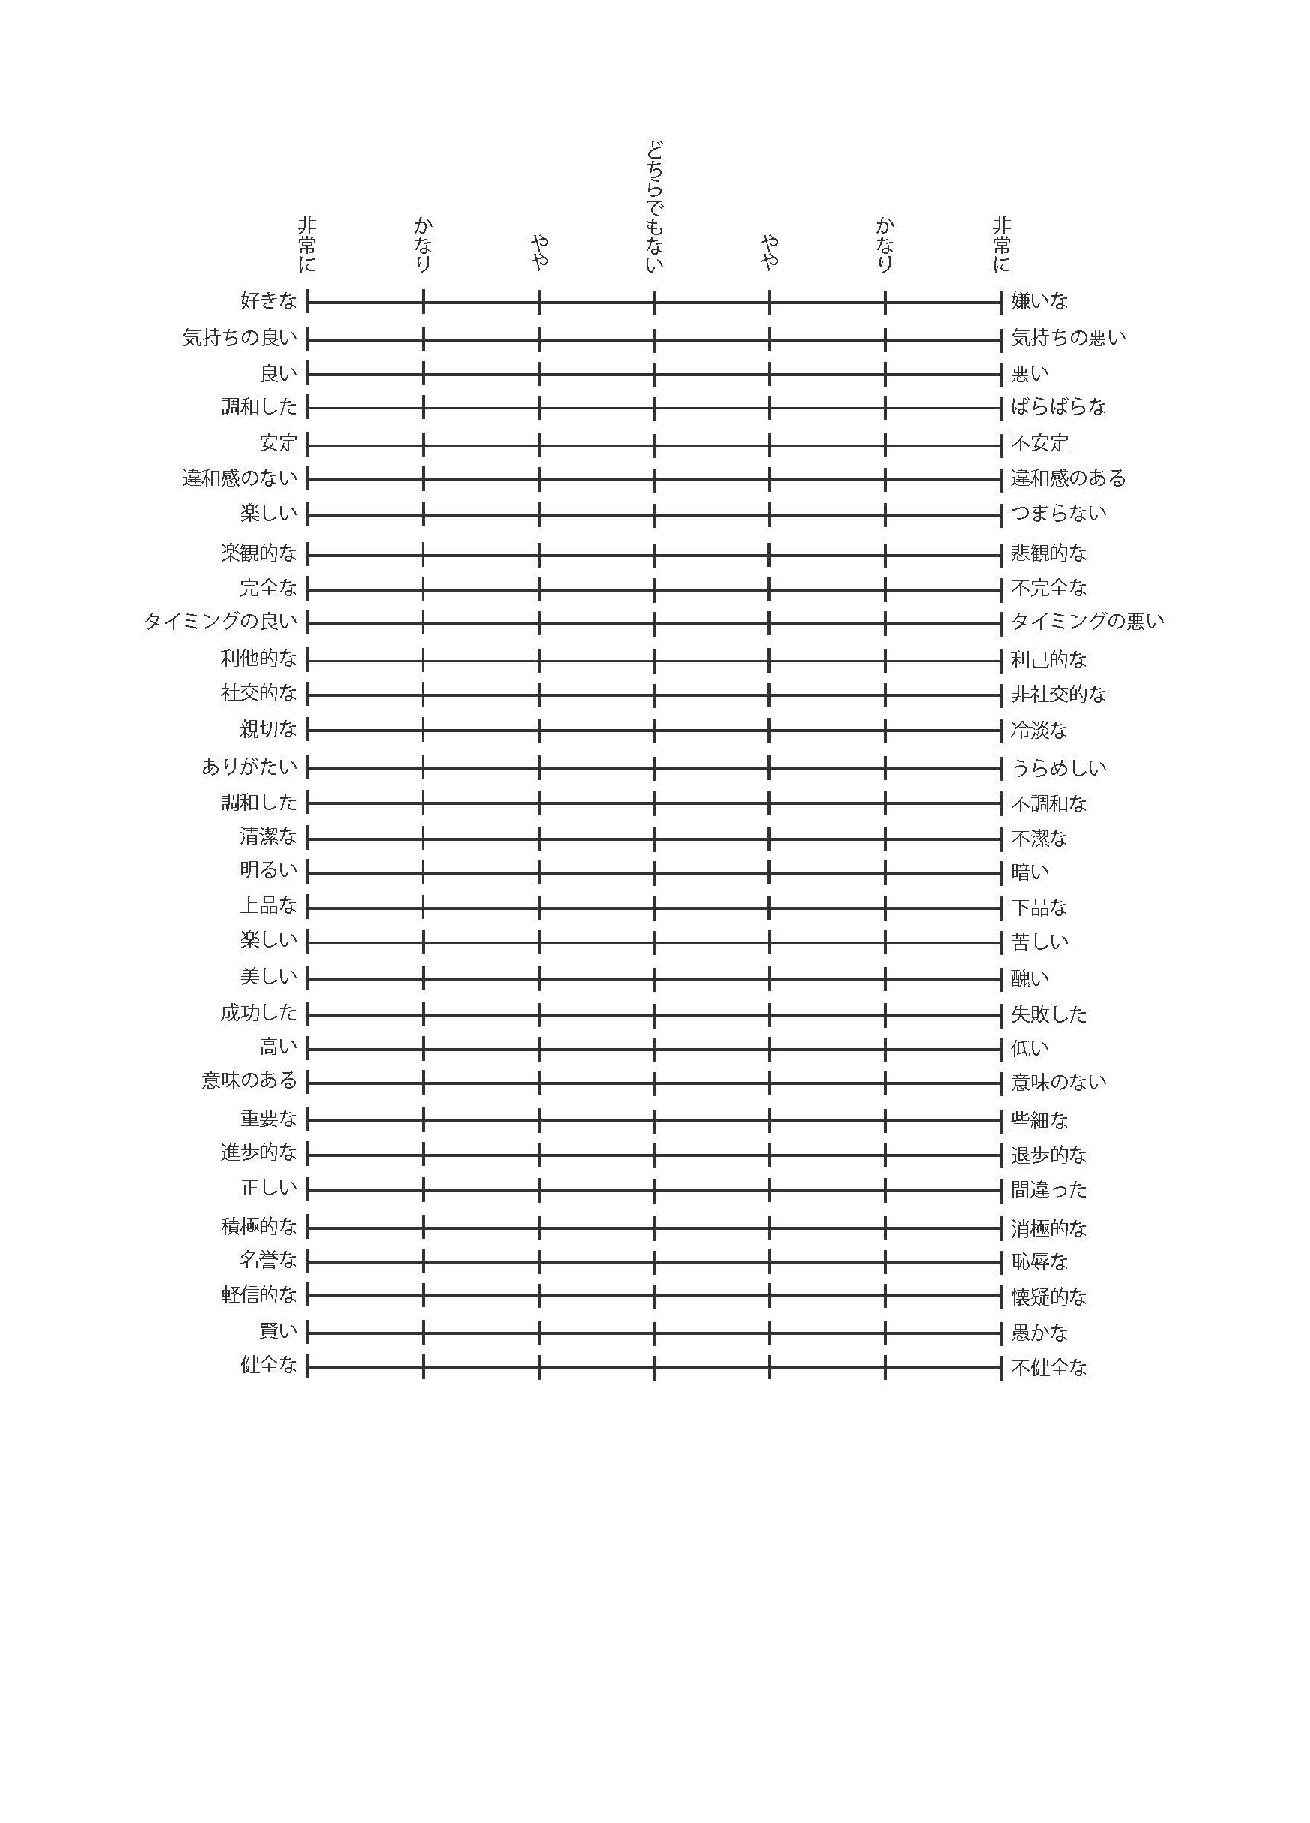
\includegraphics[width=0.9\textwidth]{chap3-figure/a-2.eps}
			}
	\caption{アンケート3枚目}
	\label{fig:ank3}
\end{figure}
\begin{figure}[tbp]
	\centering
	\fbox{
			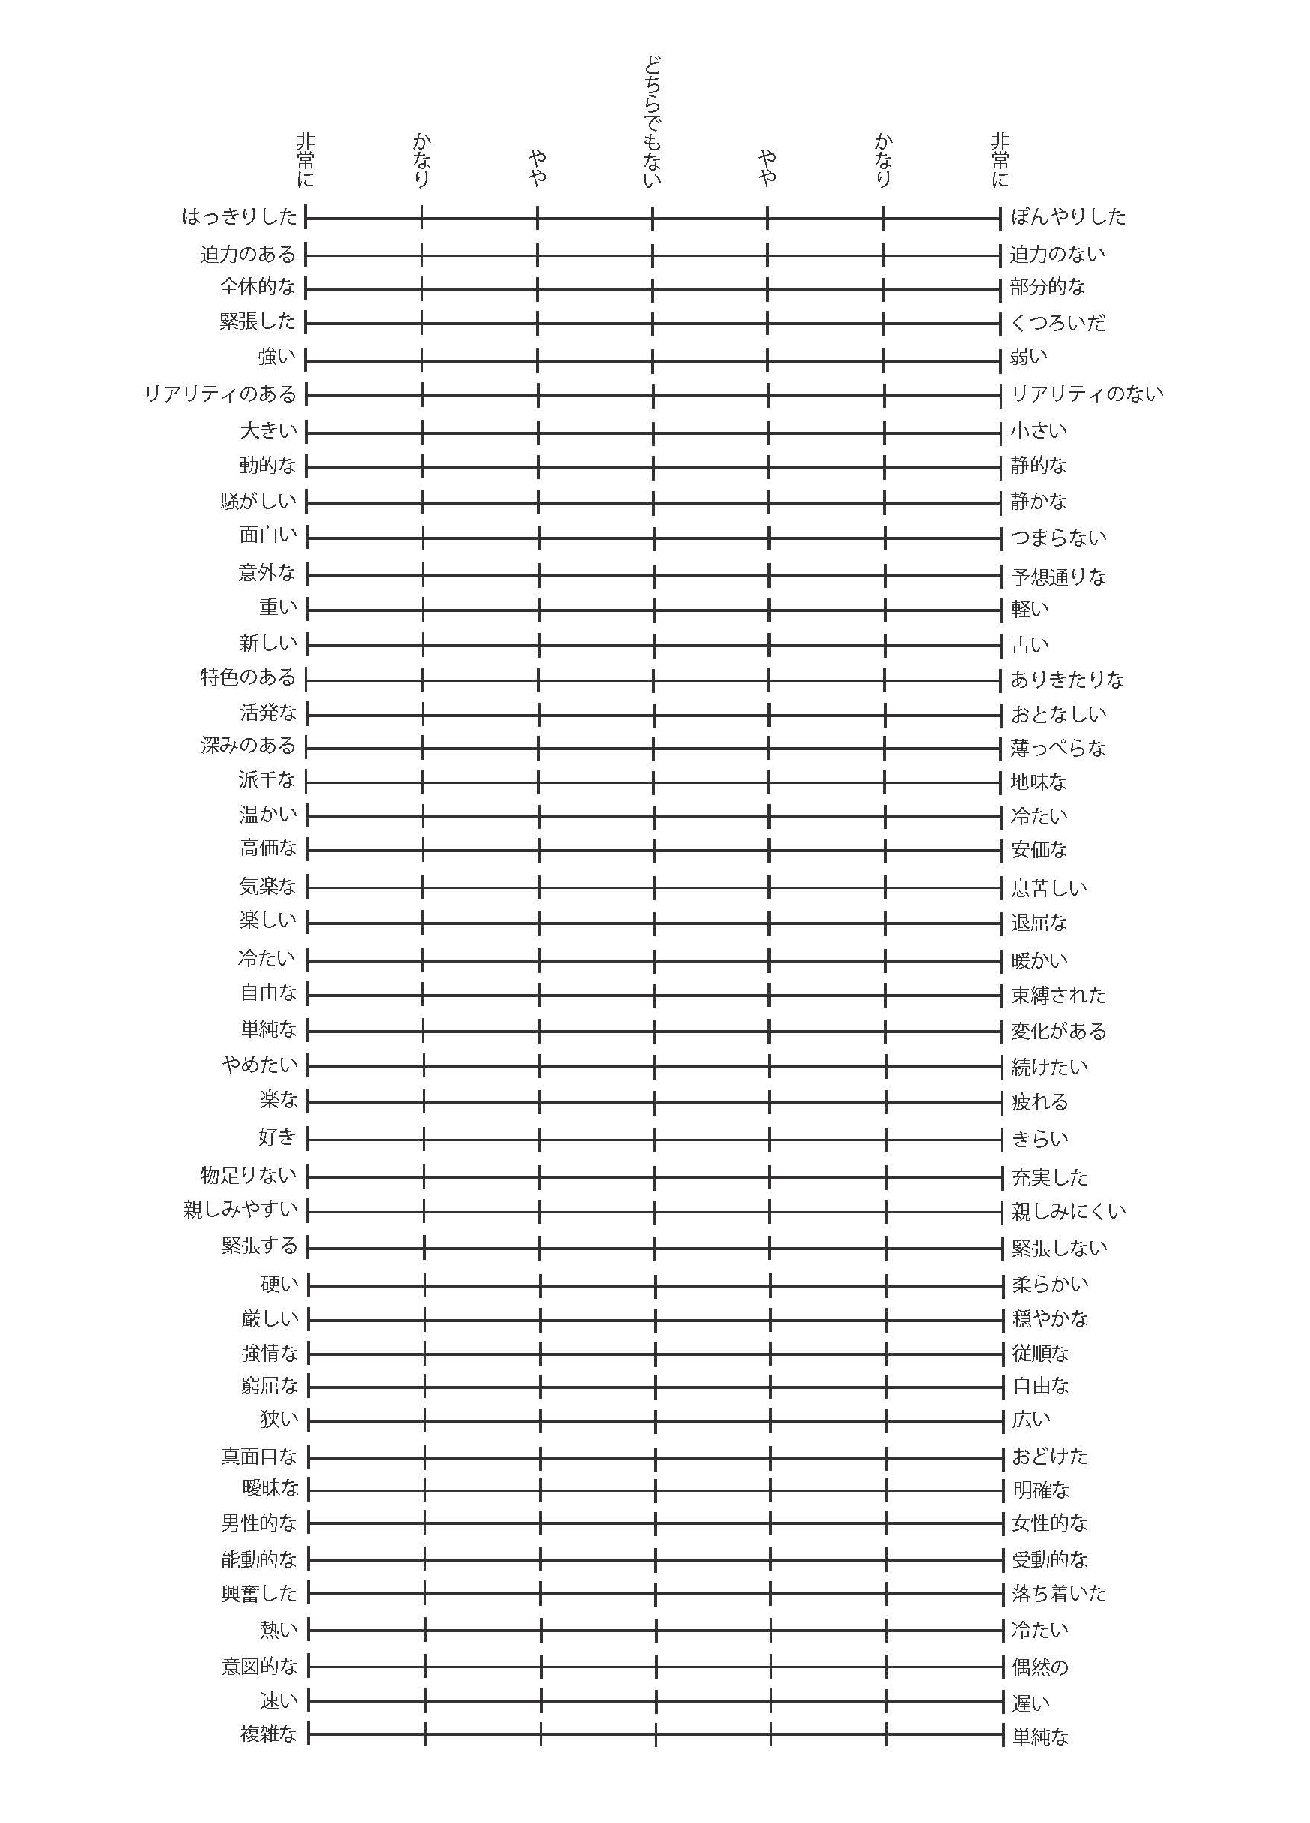
\includegraphics[width=0.9\textwidth]{chap3-figure/a-3.eps}
			}
	\caption{アンケート4枚目}
	\label{fig:ank4}
\end{figure}

\begin{figure}[tbp]
	\centering
			\includegraphics[width=0.8\textwidth]{chap3-figure/jiken.eps}
	\caption{実験風景}
	\label{fig:jiken}
\end{figure}

\begin{figure}[tbp]
	\centering
			\includegraphics[width=0.8\textwidth]{chap3-figure/ankert.eps}
	\caption{アンケート回答の様子}
	\label{fig:ankkai}
\end{figure}

\section{考察}
アンケートで得られた結果を基に考察を行う.アンケートの回答の様子を図\ref{fig:ankkai}に示す.また,自由記述の回答時間は3分間とした.

\subsection{SD法アンケート考察}
各実験およびアンケート評価の結果から考察について述べる.各実験の平均値\cite{average}を算出し,モチベーションに関わる形容詞対を抜粋し比較を行った.実験1と実験2で各形容詞対の尺度の平均値を比較し,セマンティック・プロフィール\cite{sd_zu}で図示することで提案システムによる印象の影響を調べた.

実験1と実験2を比較したアンケート結果を図\ref{fig:j-1-2}に示す.図\ref{fig:j-1-2}から実験1 と実験2を比較して,楽しい・面白い・新しい・遅い・健全な・好き,という印象が得られた.これらの結果から提案システムは好印象であることが考えられる.一方でネガティブな「遅い」という印象を解決することが今後の課題といえる.


実験1と実験3を比較したアンケート結果を図\ref{fig:j-1-3}に示す.図\ref{fig:j-1-3}から実験1 と実験3を比較して,楽しい・面白い・新しい・遅い・健全な・嫌いな,という印象が得られた.これらの結果から提案システムは好印象の面もあるが改善点もあると考えられる.一方でネガティブな「遅い」,「嫌い」という印象を解決することが今後の課題といえる.


実験1と実験4を比較したアンケート結果を図\ref{fig:j-1-4}に示す.図\ref{fig:j-1-4}から実験1 と実験4を比較して,楽しい・面白い・新しい・遅い・健全な・嫌いな,という印象が得られた.これらの結果から提案システムは好印象の面もあるが改善点もあると考えられる.一方でネガティブな「遅い」,「嫌い」という印象を解決することが今後の課題といえる.


以上の結果から,実験1の提案システムを使用した下肢リハビリがリハビに対するモチベーションの向上に繋がることが考えられる.
また,マン・ホイットニーのU検定\cite{U検定}を使用し各実験の形容詞対に有意差が見られた形容詞対を示す結果を示す.

実験1と実験2では形容詞対の有意差は確認できず,実験1と実験3では,実験1の条件のほうが「緊張する」と回答する傾向が得られた.また,実験3の条件のほうが「良い」「明るい」「迫力のある」「温かい」「熱い」と回答する傾向があった.実験1と実験4では,実験4の条件のほうが「全体的な」「能動的な」と回答する傾向が確認できた.
\begin{figure}[tbp]
	\centering
			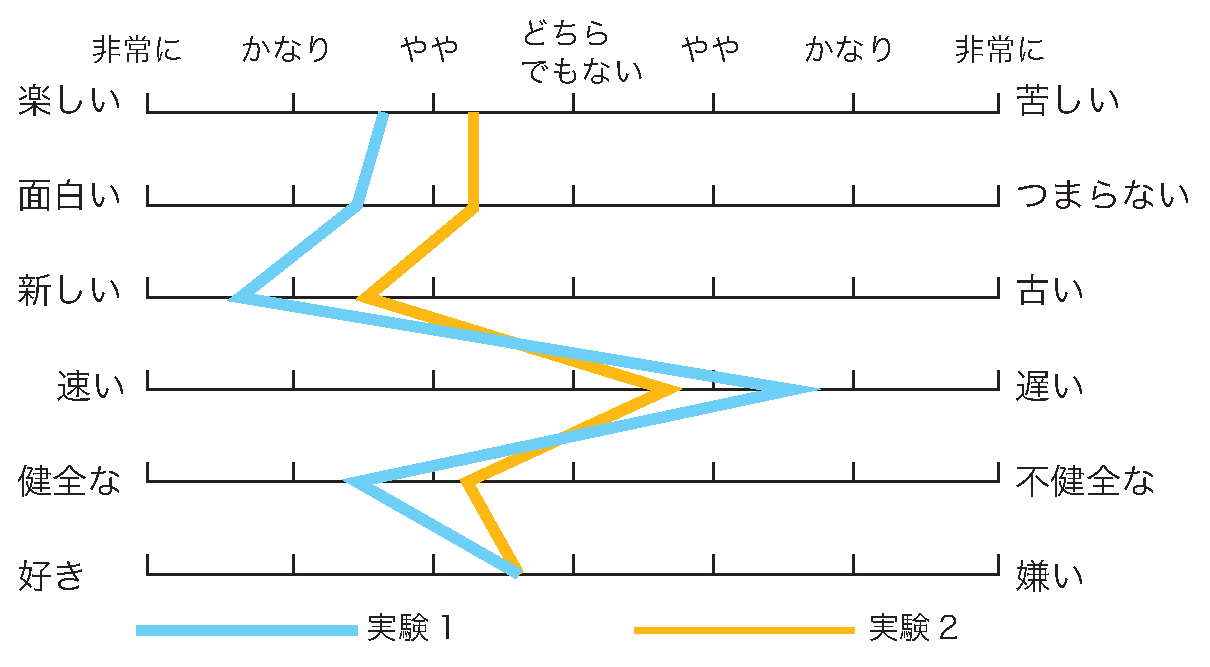
\includegraphics[width=0.9\textwidth]{chap3-figure/j-1-2.eps}
	\caption{実験1と実験2のセマンティック・プロフィール}
	\label{fig:j-1-2}
\end{figure}

\begin{figure}[tbp]
	\centering
			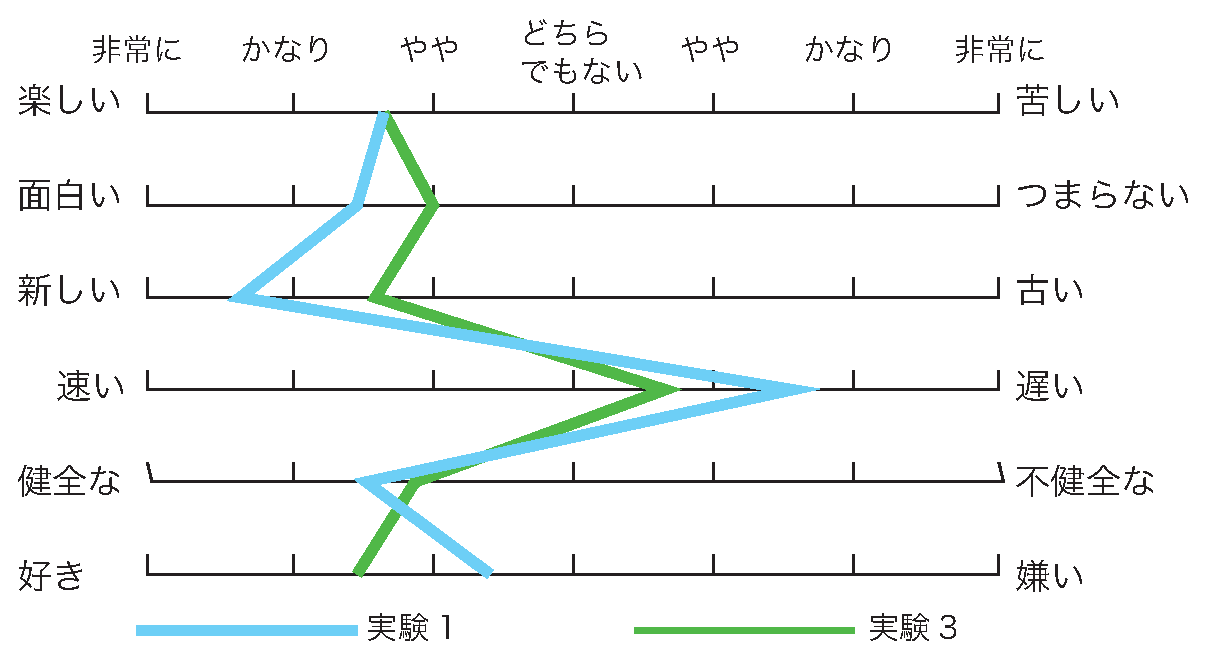
\includegraphics[width=0.9\textwidth]{chap3-figure/j1-3.eps}
	\caption{実験1と実験3のセマンティック・プロフィール}
	\label{fig:j-1-3}
\end{figure}
\begin{figure}[tbp]
	\centering
			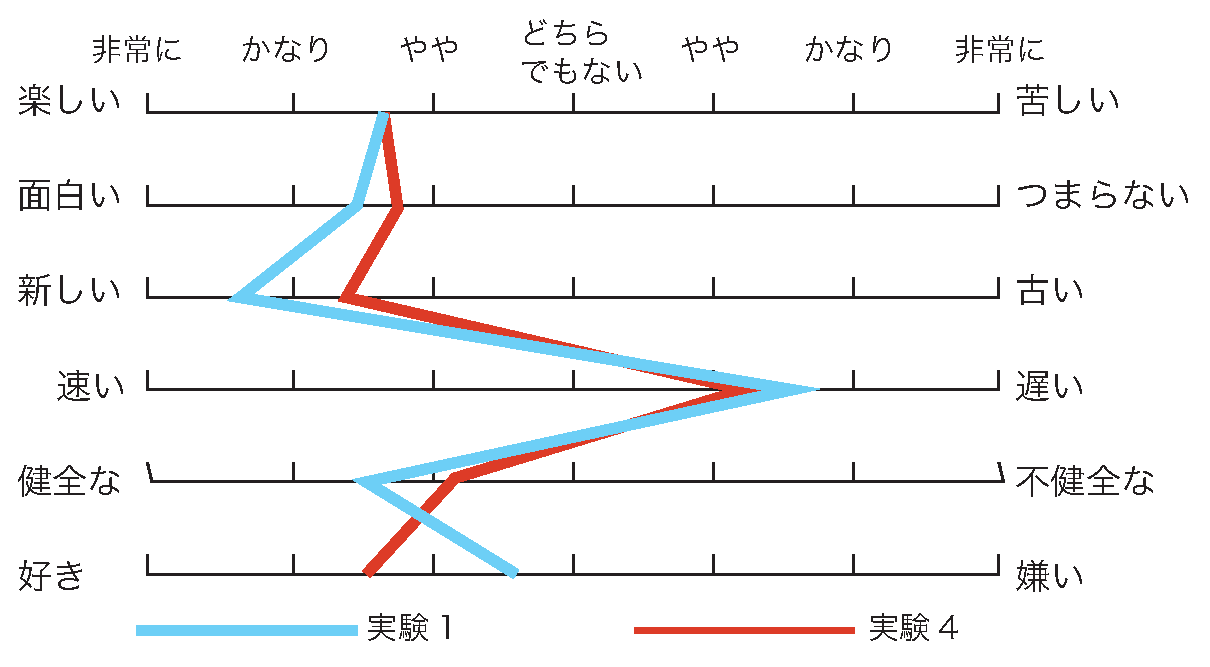
\includegraphics[width=0.9\textwidth]{chap3-figure/j1-4.eps}
	\caption{実験1と実験4のセマンティック・プロフィール}
	\label{fig:j-1-4}
\end{figure}

\subsection{自由記述アンケート考察}
自由記述アンケートを行った際の個人間の回答の主な頻出ワードを提示し,個人間の回答の傾向をつかむ.実験1の記述式アンケートの結果を図\ref{fig:j-1}に示す.図\ref{fig:j-1}から,実験1では「楽しい・面白い」や「面白い」といったリハビリに対してポジティブな意見が確認された.また,「歩いているようだ」や「足のトレーニングになりそう」といったリハビリに対するポジティブな意見も出された.

実験2の記述式アンケートの結果を図\ref{fig:j-2}に示す.図\ref{fig:j-2}から,実験2では「歩いている感じ」や「暇・他事ができそう」や「作動音がうるさい」といった意見が確認された.「作動作音がうるさい」といった意見から,被験者にヘッドフォンを着用し,生活音も出力するシステムへの変更も検討される.これにより臨場感が高まり,没入感の向上が期待できる.

実験3の記述式アンケートの結果を図\ref{fig:j-3}に示す.図\ref{fig:j-3}から,実験3では「楽しかった」や「景色が変わらないのは不自然」や「景色が綺麗」や「歩いているような」といった意見が確認された.結果から,被験者は下肢リハビリを行っているのにキャラクタの移動がないと違和感を感じる意見が確認された.

実験4の記述式アンケートの結果を図\ref{fig:j-4}に示す.図\ref{fig:j-4}から,実験4では「面白い」や「楽しい」や「ゆっくりとした」といった意見が確認された.結果から,歩行の感覚が長くゆっくりとしたといった,意見が出されたと考えられる.

\begin{figure}[!tbp]
	\centering
			\includegraphics[width=0.8\textwidth]{chap3-figure/j1.eps}
	\caption{実験1の自由記述}
	\label{fig:j-1}
\end{figure}
\begin{figure}[!tbp]
	\centering
			\includegraphics[height=0.7\textwidth]{chap3-figure/j2.eps}
	\caption{実験2の自由記述}
	\label{fig:j-2}
\end{figure}
\begin{figure}[!tbp]
	\centering
			\includegraphics[width=0.9\textwidth]{chap3-figure/j3.eps}
	\caption{実験3の自由記述}
	\label{fig:j-3}
\end{figure}
\begin{figure}[!tbp]
	\centering
			\includegraphics[width=0.9\textwidth]{chap3-figure/j4.eps}
	\caption{実験4の自由記述}
	\label{fig:j-4}
\end{figure}

\section{むすび}
本章では,提案システムの実装を行い,提案システムと他動歩行器具を被験者に対して使用したアンケート評価について述べた.そして,それぞれの実験に対しての考察を行った.

% Local Variables: 
% mode: japanese-LaTeX
% TeX-master: "root"
% End: 


%\chapter{結言}
\thispagestyle{myheadings}

\section{まとめ}
本研究では,ベッド型の下肢リハビリ装置を拡張する没入型歩行感覚提示システムを提案し,大学生の被験者に対して提案システムの印象に関するアンケート調査を行った.SD法を用いたアンケートの結果より,提案システムに対して肯定的な意見が確認され,リハビリへのモチベーション向上が期待される.今後の課題として,「作動音がうるさい」という問題点を解決するために,被験者にヘッドフォンを着用し,生活音を利用した没入感の向上が検討される.また,「歩いている距離が短い」という問題を解決するために,被験者の足の長さに合わせたCGキャラクタの移動距離の変更の実装も考えられる.
\section{今後の課題}
本節では,提案システムを使用した評価実験に基づいた今後の課題について述べる.
本研究における今後の課題として,提案システム内での音の考慮,複数人での提案システムの使用による相乗効果の検討,応用としてKinectとHMDを使用した歩行感覚提示システムの応用などが挙げられる.以下に各課題について述べる.
\subsection{音の考慮}
「寂しい」という意見やベッド型の下肢リハビリ装置の作動音がうるさいという意見があげられたので,ヘッドフォンを着用し,生活音も出力するシステムへの変更も検討される.これにより臨場感が高まり,没入感の向上が期待できる.

\subsection{歩幅の変更}
「歩いている距離が短い」という意見から,被験者の歩幅に合ったキャラクタの移動距離の変更を実装する必要が検討される.性差や各年代の歩幅を調べ性別や年齢を入力することでキャラクタの移動を変更するシステムが考えられる.

\subsection{複数人での使用による相乗効果の検討}
実験環境で使用したUnityのオンラインシステムを使用し,複数人でコミュニケーションを取りながらリハビリを行えるシステムも考えられる.
これにより,寂しさや単調さを解消が期待される.

\subsection{KinectとHMDを使用したリハビリ}
ヘルス・リテラシーの向上を目指し,「23区VRウォーキング」が開発されている.図\ref{fig:VR1}に示す,仮想空間をKinectを使用してユーザの動作を検出し,図\ref{fig:KHR-1}--\ref{fig:KHR-2}に示す足踏みの動作によってキャラクタが移動するコンテンツとなっている.そこで今回開発したHMDを使用した歩行感覚提示装置とKinectを使用し,「23区VRウォーキング」よりも没入感の高いコンテンツに応用可能と考えられる.

\begin{figure}[tbp]
	\centering
			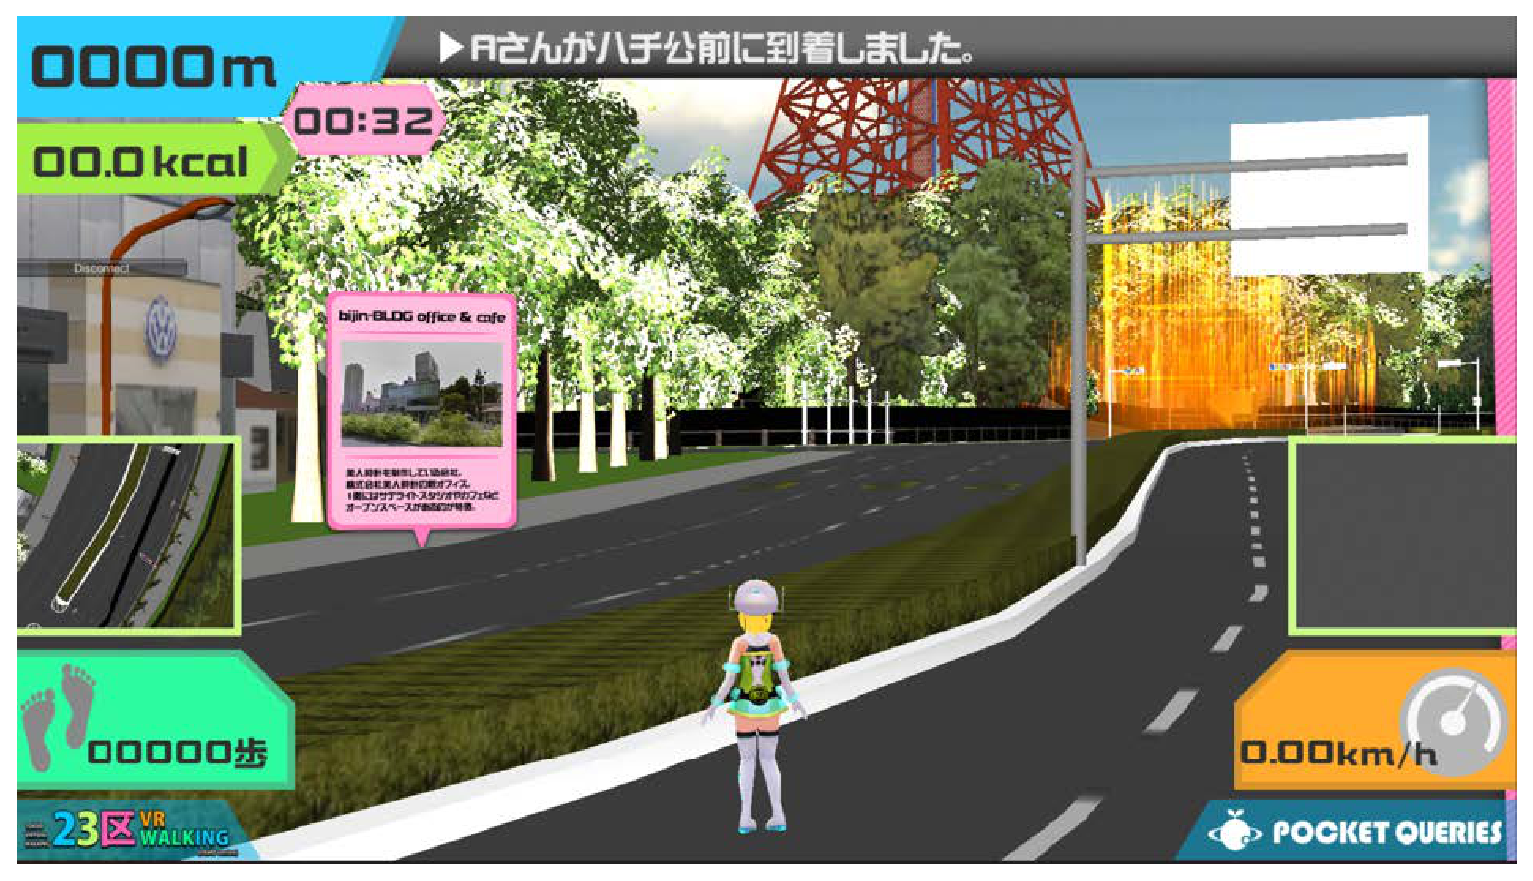
\includegraphics[width=0.9\textwidth]{chap4-figure/VR1.eps}
	\caption{関連コンテンツ(文献\cite{VR}より引用)}
	\label{fig:VR1}
\end{figure}

\begin{figure}[tbp]
	\centering
			\includegraphics[width=0.9\textwidth]{chap4-figure/kine_ocu_1.eps}
	\caption{KinectとHMDを使用した足踏みのリハビリの例(横からの図)}
	\label{fig:KHR-1}
\end{figure}
\begin{figure}[tbp]
	\centering
			\includegraphics[width=0.9\textwidth]{chap4-figure/kine_ocu_2.eps}
	\caption{KinectとHMDを使用した足踏みのリハビリの例(正面からの図)}
	\label{fig:KHR-2}
\end{figure}


% Local Variables: 
% mode: japanese-LaTeX
% TeX-master: "root"
% End: 


% \include{chap5}

%\chapter*{謝辞}
\addcontentsline{toc}{chapter}{\protect\numberline {} 謝辞}

本論文は筆者が愛知工業大学情報科学部情報科学科コンピュータシステム専攻在学中に行った研究成果をまとめたものである.
愛知工業大学情報科学部情報科学科澤野弘明准教授には研究室配属時より筆者の指導教官として,学会や他大と開催した合同シンポジウムに参加する機会を与えて下さるともに,日頃より多くのご指導ご鞭撻を賜りましたことを,ここに心から深く感謝致します.また愛知工業大学情報科学部情報科学科の教授,准教授,講師の方々には,大学入学時より多くのご指導ご鞭撻を賜りまして,心から感謝致します.研究の協力・支援をしてくださった,中部大学の尾方寿好先生,鈴木裕利先生,愛知きわみ看護短期大学の石井成郎先生に,深く感謝致します.また,日頃から活発な議論にお付き合い頂き,助言を頂いた,愛知工業大学大学院経営情報科学研究科澤野研究室に所属している小西拓也氏,原拓海氏,山田郷史氏,岩本雄太氏,林友貴氏に感謝致します.%獣の狩人・サンダ大先生(@xxSANDAxx)氏に感謝致します.
研究室配属時から研究に関する実験の実施や助言を頂いた,有限会社サイバーネットワークス社長の立野雄也氏,愛知工業大学情報科学部情報科学科澤野研究室の井嶋亮太氏,畑広貴氏,山口達也氏,浅井美香氏,伊神栞里氏,加藤葵氏,加藤晃哉氏,栗原春菜氏,小山直紀氏,佐藤貴明,佐分基泰氏,志賀俊佑氏,前田拓磨氏,浅野拓也氏,岡田伊織氏,澤田和伸氏,栗原尚弘氏に深く感謝致します.

% Local Variables: 
% mode: latex
% TeX-master: "root"
% End: 


\thispagestyle{myheadings}
\markboth{参考文献}{参考文献}
\markright{}
\def\bibname{参考文献}
\begin{thebibliography}{20}

\addcontentsline{toc}{chapter}{\protect\numberline {}参考文献}

\bibitem{認知症とは}
日本神経学会: ``認知症疾患治療ガイドライン2010'', pp. xx--xx (20xx)

\bibitem{認知症予防マニュアル}
国立長寿医療研究センター: ``認知症予防マニュアル'', pp. 6--8 (2011)

\bibitem{高齢社会白書}
内閣府: ``平成29年版高齢社会白書'', pp. xx--xx (2017)

\bibitem{新オレンジプラン}
厚生労働省: ``認知症施策推進総合戦略(新オレンジプラン)'', pp. xx--xx (20xx)

\bibitem{運動の効果}
島田裕介: ``認知症予防を目的とした運動の効果'', 理学療法学, Vol. 42, No. 4, pp. 341--342 (2015)

\bibitem{運動教室}
重松良祐,大久保善郎,大須賀洋祐,中田由夫,根本みゆき,沖直哉,田中喜代次: ``運動中心の介護予防教室を修了した高齢者のための受け皿事業'', 厚生の指標, Vol. 62, No. 2, pp. 7--14 (2015)

\bibitem{コグニサイズとは}
国立長寿医療研究センター: ``コグニサイズとは?'', \url{http://www.ncgg.go.jp/cgss/department/cre/cognicise.html}(confirmed in Feb. 2017)

\bibitem{国立長寿医療研究センター}
国立長寿医療研究センター: \url{http://www.ncgg.go.jp/cgss/department/cre/cognicise.html}(confirmed in Feb. 2017)

\bibitem{認知症予防へ向けた運動コグニサイズ}
国立長寿医療研究センター: ``認知症予防へ向けた運動コグニサイズ'', pp. xx--xx (20xx)

\bibitem{運動教室の効果}
滝本幸治, 宮本謙三, 竹林秀晃, 井上佳和, 宅間豊, 古谷信之, 宮本祥子, 岡部孝生: ``地域に根ざした高齢者運動教室の効果検証'', 理学療法学, Vol. 24, No. 2, pp. 281--285 (2009)

\if0
\bibitem{理学療法士}
国内渉外部: ``作業療法士の需給計画の 見直し'', 理学療法学, Vol. 18, No. 6, pp. 645-657 (1991)

\bibitem{フィットネスマシン}
竹井機器工業株式会社: ``ゲーム機能を搭載した施設向けフィットネスマシンを開発'', 報道発表資料 (2010)
\url{http://www.takei-si.co.jp/productinfo/detail/pdf/puresu.pdf}(confirmed in Feb. 2016)
\bibitem{歩行イメージ再学習}
大橋麻美, 保坂章夫, 岡田利香, 久保通宏, 関根由里, 古谷信之, 増岡泰三, 後藤博: ``脳卒中急性期片麻痺患者における歩行イメージ再学習後の歩容変化'', 理学療法学, Vol. 32,  pp. 441 (2005)

\bibitem{筑波歩行感覚提示}
田中直樹, 斉藤秀之, 飯塚陽, 矢野博明, 奥野純子, 柳久子: ``維持期脳卒中患者に対する歩行感覚提示装置を用いた歩行トレーニング効果の持続性'', 理学療法科学, Vol. 27,No.2, pp. 123--128 (2012)

\bibitem{筑波歩行感覚提示画像}
国立研究開発法人新エネルギー・産業技術総合開発機構: ``リハビリ患者がより現実に近い移動感覚で歩行機能の改善訓練ができる装置と訓練中の飽きを防ぎリハビリ効果の向上を実現する球面ディスプレイを組み合わせた新しい歩行リハビリテーションシステムの開発'', 成果事例集原稿, p. 3 (2008)

\bibitem{日立}
藤江正克, 土肥健純, 根本泰弘, 酒井昭彦, 吉田輝, 佐久間一郎, 鈴木真,``参加支援工学 バーチャルリアリティを活用した歩行訓練機器'', 日本生体医工学会, Vol. 12, No. 8, pp. 29--37 (1998) 

\bibitem{ディスプレイの違い}
小林秀明,浅井紀久夫: ``歩行動作環境において提示ディスプレイの違いが感性に与える影響'', ヒューマン情報処理, Vol. 105, pp. 143--148 (2005)

\bibitem{ロコモーション}
野間春生: ``ロコモーションとバーチャルリアリティ'', 社団法人 計測自動制御学会, Vol. 143, No. 2, pp. 133--138 (2004)

%\bibitem{足踏み}
%針山拓人, 大倉典子: ``足踏みによる歩行感覚体感デバイスの開発'', 自動制御連合講演会講演論文集, Vol.  51, pp. 223 (2008)
\bibitem{KinectV2}
KinectV2: \url{https://dev.windows.com/en-us/kinect/develop}(confirmed in Feb. 2016)

\bibitem{OculusRift}
OculusRift: \url{https://www.oculus.com/ja/rift/}(confirmed in Feb. 2016)

\bibitem{Unity}
Unity: \url{http://japan.unity3d.com/}(confirmed in Feb. 2016)

\bibitem{3D都市モデル}
Unity向け3D都市モデルデータ: \url{http://www.zenrin.co.jp/product/service/3d/asset/} (confirmed in Feb. 2016)

\bibitem{人間工学ガイド}
福田忠彦研究室: ``増補版 人間工学ガイド--感性を科学する方法--'' , サイエンティスト社, pp. 125--173 (2009)

\bibitem{average}
中村永友,山田智哉,金明哲: ``Excelで学ぶ統計\UTF{2022}データ解析入門'', 丸善株式会社 (2011).

\bibitem{sd_zu}
和田有史,續木大介,山口拓人,木村敦,山田寛,野口薫,大山正: ``\UTF{FFFC}\UTF{FFFC}\UTF{FFFC}\UTF{FFFC}\UTF{FFFC}\UTF{FFFC}\UTF{FFFC}\UTF{FFFC}\UTF{FFFC}\UTF{FFFC}\UTF{FFFC}\UTF{FFFC}\UTF{FFFC}\UTF{FFFC}\UTF{FFFC}\UTF{FFFC}\UTF{FFFC}\UTF{FFFC}\UTF{FFFC}\UTF{FFFC}\UTF{FFFC}\UTF{FFFC}\UTF{FFFC}SD法を用いた視覚研究知覚属性と感情効果の研究を例として'', VISION, Vol. 15, No. 3, pp. 179--188 (2003).

\bibitem{U検定}
Wilcoxonの順位和検定(マン・ホイットニーのU検定): \url{ http://www.gen-info.osaka-u.ac.jp/MEPHAS/wilc1.html} (confirmed in Feb. 2016)

\bibitem{VR}
株式会社ポケットクエリーズ: ``ゲームのちからの VRソリューションへの応用 〜 ジオ + VR + ゲーム = ヘルスケアソリューション 〜	'', Unity Solution Conference 2014 発表資料 (2014)
\url{http://japan.unity3d.com/events/usc2014/pdf/1300_ROOM1a_PocketQueries.pdf} (confirmed in Feb. 2016)
\fi

\end{thebibliography}
\hspace{15pt}

% これ以降,付録となる
\appendix

%\chapter{論文表紙}
\thispagestyle{myheadings}

\vspace{-1.0cm}

\begin{center}

{\LARGE 愛知工業大学情報科学部情報科学科\\
コンピュータシステム専攻

\vspace{1.0cm}

平成27年度~卒業論文\\

\vspace{2.0cm}

{\Huge 
\baselineskip=15mm
\textbf{\\他動歩行リハビリ装置を拡張する
\\没入型歩行感覚提示による視覚刺激に
\\関する研究\\}}

\vspace{7.0cm}

2016年2月\\

\vspace{1.0cm}

\begin{tabular}[h]{lll}
  研究者 & K12031 & 片桐雅貴\\
\end{tabular}

\vspace{1.0cm}

指導教員\ \ 澤野弘明\ \ 准教授}

\end{center}

% Local Variables: 
% mode: latex
% TeX-master: "root"
% End: 


\end{document}

%%% Local Variables: 
%%% mode: latex
%%% TeX-master: t
%%% End: 
